\documentclass[
  ngerman,
  a4paper,
  12pt
]{report}

\usepackage[utf8]{inputenc}
\usepackage[english, german]{babel}
\usepackage[left=2.5cm, right=2.5cm]{geometry}
\usepackage{csquotes}
\usepackage{setspace}
\usepackage{caption}
\usepackage{xparse}
\usepackage[dvipsnames]{xcolor}
\usepackage{siunitx}
\usepackage{booktabs}

\usepackage{enumitem}
\setlist{itemsep=0pt}

\usepackage{tikz}
\usetikzlibrary{positioning, calc, arrows.meta, shapes.multipart, fit}
\usepackage[cache=false]{minted}
\renewcommand{\listingscaption}{Quelltext}
\renewcommand{\listoflistingscaption}{Quelltextverzeichnis}

\setminted{
  autogobble,
  xleftmargin=2em,
  fontsize=\scriptsize,
  formatcom=\onehalfspacing\fontencoding{T1}\fontfamily{fvm}\selectfont,
}

\newmintinline{python}{
  style=custompy,
}
\newminted{python}{
  style=custompy,
}
\newmintinline{pycon}{
  style=custompy,
}
\newminted{pycon}{
  style=custompy,
}
\newminted{console}{
  style=customshell
}
\newmintinline{console}{
  style=customshell
}

\AtBeginEnvironment{consolecode}{\color[HTML]{191565}}
\newcommand{\yhat}{\hat{y}}
\newcommand{\zB}{z.\,B.}
% \newcommand{\cpp}{C\texttt{++}}
\newcommand{\cpp}{{C\nolinebreak[4]\hspace{-.05em}\raisebox{.4ex}{\tiny\bf ++}}}
\newcommand{\wSM}{0.6\textwidth}
\newcommand{\wMD}{0.65\textwidth}
\newcommand{\wLG}{0.7\textwidth}
\newcommand{\wXL}{0.75\textwidth}
\newcommand{\wXXL}{0.80\textwidth}
\newcommand{\wXXXL}{0.85\textwidth}

\makeatletter
\renewcommand{\paragraph}{%
  \@startsection{paragraph}{4}{\z@}%
  {1.5ex \@plus 1ex \@minus .2ex}{-1em}%
  {\normalfont\normalsize\bfseries}%
}
\makeatother

\usepackage[unicode]{hyperref}
\hypersetup{
  linkcolor = Red,
  filecolor = Magenta,
  urlcolor = Green,
  citecolor = Cyan
}
\urlstyle{same}

\usepackage{amsmath}

\usepackage[style = authoryear-ibid]{biblatex}
\addbibresource{preamble/main.bib}

\usepackage{graphicx}
\graphicspath{{./images}}

\usepackage[tikz]{mdframed}

\NewDocumentEnvironment{aquote}{m}
  {\begin{quote}}
  {\\\hspace*{16pt}--- #1\end{quote}}

\begin{document}
\pagenumbering{Roman}
\newcommand{\SiemensLogo}{
\includegraphics[width=4cm]{images/siemens-logo.png}}
\newcommand{\DhbwLogo}{
\includegraphics[width=4cm]{images/dhbw-logo.png}}
\newcommand{\Titel}{Ein Verteiltes Systeme für mobiles Maschinelles Lernen}
\newcommand{\Was}{Bachelorarbeit}
\newcommand{\Abschluss}{Bachelor of Science}
\newcommand{\Studiengang}{Informatik / Angewande Informatik}
\newcommand{\Author}{\textbf{Jens Döllmann}}
\newcommand{\Abgabedatum}{30. August 2021}

\newcommand{\Dauer}{3 Monate}
\newcommand{\Matrikelnummer}{8876462}
\newcommand{\Kursbezeichnung}{TINF18B4}
\newcommand{\FirmenName}{Siemens AG}
\newcommand{\FirmenStadt}{Karlsruhe}
\newcommand{\BetreuerFirma}{Florian Seiter}
\newcommand{\BetreuerDHBW}{Gerhard Wolf}

\begin{titlepage}
  \begin{center}
    \huge
    \vspace*{-2cm}
    \SiemensLogo \hfill \DhbwLogo\\[2cm]
    \Titel\\[1cm]
    {\scshape \Was}\\[1cm]

    \large
    für die Prüfung zum\\[0.5cm]
    \Abschluss\\[0.5cm]
    des Studiengangs \Studiengang\\[0.5cm]
    an der\\[0.5cm]
    Dualen Hochschule Baden-Württemberg Karlsruhe\\[0.5cm]
    von\\[0.5cm]
    \Author\\[1cm]
    Abgabedatum \Abgabedatum
  \end{center}

  \vfill

  \begin{tabular}{l@{ \hspace{2cm} }l}
    Bearbeitungszeitraum          & \Dauer           \\
    Matrikelnummer                & \Matrikelnummer  \\
    Kurs                          & \Kursbezeichnung \\
    Betreuer der Ausbildungsfirma & \BetreuerFirma   \\
    Gutachter der Studienakademie & \BetreuerDHBW    \\
  \end{tabular}
\end{titlepage}
\onehalfspacing
\include{pages/erklärung.tex}
\newenvironment{abstractpage}
{\cleardoublepage\vspace*{\fill}\thispagestyle{empty}}
{\vfill\cleardoublepage}
\newenvironment{myabstract}[1]
{\bigskip\selectlanguage{#1}
  \begin{center}
    \bfseries\abstractname
  \end{center}}
{\par\bigskip}

\begin{abstractpage}
\begin{myabstract}{german}
In dieser Arbeit geht es um den Entwicklungsprozess einer Anwendung
für mobiles Maschinelles Lernen. Zusammen mit Google Coral Edge TPUs
(\textit{Tensor Processing Units})
wird die Architektur eines Systems vorgestellt, mit dem
neuronale Netze auf verteilten Geräten ausgeführt
und Netzergebnisse kommuniziert werden.
Hierfür wird damit begonnen, die Geschichte der Künstlichen Intelligenz
zu untersuchen, um anschließend einen Einstieg in das Gebiet
von Deep Learning zu geben. Mithilfe von TensorFlow wird
gezeigt, wie ein neuronales Netz trainiert
und auf mobilen und eingebetteten Geräten bereitgestellt wird.
Des Weiteren wird hierbei die Integration mit der Edge TPU besprochen
und Testergebnisse in Bezug auf Genauigkeit und Inferenzgeschwindigkeit
dokumentiert. Die Ausführung auf der Edge TPU erzeugt keine
oder nur kaum bemerkbare Genauigkeitsverluste, jedoch ist die Geschwindigkeit
in den durchgeführten Benchmarks
langsamer als die gleiche Ausführung auf der CPU.
Mögliche Auslöser für dieses Ergebnis können schließlich diskutiert werden.
\end{myabstract}
\begin{myabstract}{english}
This thesis deals with the development process of building
an application for mobile Machine Learning.
Using Google Coral Edge TPUs (tensor processing units)
we describe a distributed system
for querying neural networks wrapped in a service.
We will start by examining the history of Artificial Intelligence
and then give an introduction into the field of Deep Learning.
With the help of TensorFlow, we show the process of training a
simple neural network and how to deploy the model to
a mobile device. Moreover, both models are compared.
Inference on the Edge TPU does not reduce the model's accuracy.
However, when benchmarking the performance,
the model performed slower than when running on the CPU.
Finally, we discuss possible triggers for this behaviour.
\end{myabstract}
\end{abstractpage}
\tableofcontents
\listoffigures
\listoftables
\newpage
\pagenumbering{arabic}
\chapter{Einleitung}
Hören die meisten Personen die Begriffe \enquote{Künstliche Intelligenz}
und \enquote{Maschinelles Lernen} stellen sie sich Roboter vor:
treue Diener, die all deine Aufgaben übernehmen oder eine tödliche Arme
von superintelligenten Cyborgs im Kampf gegen die Menschheit.
Künstliche Intelligenz (kurz KI) ist jedoch schon lange nicht mehr nur eine futuristische
Fantasie und Teil von Science-Fiction-Filmen; es wird bereits großflächig
eingesetzt und findet Verwendung in einer Vielzahl von Anwendungen aus Bereichen
in nahe zu allen Teilen der Wirtschaft. Andrew Ng,
welcher unteranderem durch seine beliebten Onlinekurse zum Thema
Maschinellen Lernen (ML) und Deep Learning (DL)
bekannt ist,
\footnote{\url{https://www.coursera.org/instructor/andrewng}}
vergleicht KI mit der neuen Elektrizität.
\begin{aquote}{Andrew Ng \parencite{online:ai-andrew-ng}}
  \enquote{\textit{Just as electricity transformed almost everything 100 years ago,
      today I actually have a hard time thinking
      of an industry that I don’t think AI will
      transform in the next several years}}
\end{aquote}
Die Anwendung, mit der Maschinelles Lernen erstmalig öffentliche Aufmerksamkeit
erlangte und und noch immer das tägliche Leben vieler Menschen beeinflusst,
stammt aus den 90er-Jahren:
Die Rede ist von dem E-Mail-Spamfilter \parencite[1]{book:hands-on-ml}.
Es handelt sich um eine scheinbar einfache Aufgabe, welche
mit traditioneller Programmierung aber dennoch nur schwer gelöst werden kann.
Ein klassisches Programm besteht aus vielen statischen Regeln,
im Fall des Spamfilters können diese dazu dienen, auffällige Schlüsselwörter und
Satzteile zu erkennen (wie \enquote{Kreditkarte}, \enquote{konstenlos}, \enquote{kaufen} oder
andere Merkmale).
Ein statisches Programm ist nicht gut dafür geeignet, ein dynamisches Problem
zu beschreiben. Die Absender der Spamnachrichten könnten erkennen, welche E-Mails blockiert werden
und diese leicht abändern. Arbeiten sie so durchgehend um das Problem herum,
müssen immer wieder neue Regeln im Programm aufgenommen werden. Ein Spamfilter hingen,
welcher auf Maschinellen Lernen basiert, kann diese Regeln
selbstständig erkennen und automatisch anpassen wenn es eine Veränderung erkennt.
Der Algorithmus durchläuft eine Trainingsphase und verwendet dabei
Beispiel E-Mails (z.\,B. diese, die vom Benutzer markiert wurden)
und kann so lernen Spamnachrichten zu unterscheiden.
Diese Trainingsdaten werden als Trainingsdatensatz (engl. \textit{train set})
bezeichnet.
Es folgt ein Programm, welches weitaus kürzer,
einfacher zu verwalten und wahrscheinlich auch präziser ist.

\section{Was ist Maschinelles Lernen?}
Maschinelles Lernen ist die Wissenschaft (und Kunst) der Programmierung,
die es dem Computer ermöglicht, von Daten zu lernen. Arthur Samuel und Tom Mitchell
haben im Jahr 1959 und 1997 eine allgemeine und formale Definition gegeben \parencite[2]{book:hands-on-ml}:
\begin{aquote}{Arthur Samuel, 1959}
  \enquote{\textit{Machine Learning is the field of study that gives computers
      the abilty to learn without being explicitly programmed.}}
\end{aquote}
\begin{aquote}{Tom Mitchell, 1997}
  \enquote{\textit{A computer program is said to learn from experience
      $E$ with respect to some task \,$T$ and some performance measure $P$,
      if its performance on $T$, as measured by $P$, improves with experience $E$.}}
\end{aquote}
Betrachten wir erneut das Beispiel des Spamfilters, dann ist die Aufgabe $T$
das Markieren von Spam, die Erfahrung
$E$ sind die Trainingsdaten ist und der Bewertungsmaßstab $P$ bleibt zu definieren.
Es könnte zum Beispiel der Anteil der als richtig markierten E-Mails verwendet
werden. Dieser Maßstab heißt Genauigkeit und wird
häufig verwendet wenn es darum geht eine Klassifizierungsaufgabe zu bewerten.

\section{Die unterschiedlichen Lernmethoden}
\label{sec:lernmethoden}
Maschinelles Lernen kann genutzt werden, um eine Vielzahl von Problemen zu lösen.
Dies macht es zu einem mächtigen Werkzeug, aber auch eines, in dem es schwierig sein
kann, den Überblick zu behalten.
Da es viele verschiedene Architekturen und Lösungsansätze gibt, ist es sinnvoll,
diese in grobe Kategorien zu unterteilen.
Ein System kann unterschieden werden, basierend auf den folgenden
Kriterien \parencite[7]{book:hands-on-ml}:
\begin{itemize}
  \item Trainiert das System mit oder ohne menschlicher Betreuung, dann ist
        die Rede vom überwachten und unüberwachten Lernen.
  \item Kann das System inkrementell mit einer Teilmenge der Trainingsdaten
        lernen oder verwendet es die gesamten Daten. Dieser Unterschied
        nennt sich Online- vs. Batch-Learning.
  \item Funktioniert das System indem es lediglich neue Daten mit
        den alten vergleicht oder kann es Muster erkennen
        und ein prädiktives Modell entwerfen.
        Dieser Unterschied nennt sich instanzbasiertes und modellbasiertes Lernen.
\end{itemize}
Keine der eben beschriebenen Kriterien schließen sich aus.
In einem echten System können
kombinierte Lernmethoden sinnvoll sein, um das gewünschte Ergebnis zu erzielen.
Wir können nun die einzelnen Lernmethoden etwas genauer untersuchen.

\subsection{Überwachtes und Unüberwachtes Lernen}
Das überwachte und unüberwachte Lernen unterscheidet
sich darin, in welcher Form die Trainingsdaten vorliegen.
Überwachtes Lernen bedeutet, dass die Zielwerte der Daten bekannt
sind. Diese Werte werden als Label bezeichnet. Unüberwachtes Lernen
kann auch mit unbeschrifteten Daten umgehen, jedoch sind die Ziele
der beiden Verfahren meist unterschiedliche.
Labels können wie im Falle des
Spamfilters vom Benutzer stammen oder durch Naturgesetzte und Expertenwissen
gegeben sein. Obwohl die große Mehrheit der heutigen Daten unbeschriftet sind,
beschäftigen sich die meisten Algorithmen mit überwachten Lernen
\parencite[235]{book:hands-on-ml}.
Die Erstellung eines ausreichend großen, beschrifteten Datensatzes
ist eine der größten Herausforderungen im Maschinellen Lernen.

\subsection{Batch-Learning und Online-Learning}
Ein weiterer Punkt, anhand dessen ein System unterschieden
werden kann, ist die Methode, wie es Daten verarbeitet \parencite[15]{book:hands-on-ml}.
Dieser Unterschied nennt sich Batch- und Online-Learning.
Beim Batch-Learning werden die Daten stapelweise verarbeitet.
Das Modell bzw. die Parameter werden erst dann angepasst,
nachdem der gesamte Stapel (Batch) das Training durchlaufen hat.
Dies braucht in der Regel viel Zeit und Speicherkapazität, weshalb
es typischerweise offline durchgeführt wird.
Nachdem ein System veröffentlicht wurde, wendet es, dass an, was es gelernt hat,
kann aber keine neuen Schlüsse mehr ziehen.
Soll das System auf neue Daten reagieren, muss ein neues Modell trainiert werden.
Das Online-Learning funktioniert anders.
Im Training werden die Daten nicht mehr stapelweise verarbeitet,
sondern einzeln nacheinander.
Dies spart Zeit und Platz und kann hilfreich sein, wenn es darum geht,
mit sehr großen Datensätzen zu trainieren, die nicht alle gleichzeitig
in den Speicher passen würden.
Ein weiterer Vorteil ist der, dass neue Daten spontan auf dem Weg
verarbeitet werden können. Online-Learning eignet sich also gut,
um kontinuierliche Daten zu analysieren (z.\,B. Aktienkurse)

\subsection{Instanzbasiertes Lernen}
Die wohl leichteste Form des Lernens ist das einfache auswendig Lernen.
Ein Spamfilter, der nach diesem Prinzip arbeitet, würde jede E-Mail,
die identisch zu einer bereits zuvor markieren E-Mail ist erneut als Spam markieren.
Dieses Prinzip nennt sich instanzbasiertes Lernen. Um das System zu
verbessern, könnte der Algorithmus versuchen, nicht nur gleiche,
sondern auch ähnliche E-Mails zu erkennen.
\subsection{Modellbasiertes Lernen}
Das bisherige Spamfilter Beispiel ist ein typisches
Klassifizierungsproblem. Zu einer Menge von eine Eingabewerten
(auch genannt Features) soll die Wahrscheinlichkeit bestimmt werden,
dass diese Feature zu einer bestimmten Klasse gehören.
Was ist aber wenn keine Wahrscheinlichkeiten
prognostiziert werden sollen, sondern numerische Werte wie
der Preis eines Autos? Dieses Problem nennt sich Regression und
ist eine modellbasierte Lernaufgabe.
Ein Beispiel soll zeigen, wie das Prinzip funktioniert.
Das Ziel ist einfaches Modell, welches linear aussehende Daten modelliert.
Als erster Schritt müssen die Trainingsdaten generiert werden.
Der folgende Python Code zeigt diesen Vorgang mithilfe von NumPy:
\begin{pythoncode}
import numpy as np
rng = np.random.default_rng(42)
x = 6 * rng.random((100, 1))
y = 5 + 3 * x
\end{pythoncode}
NumPy ist eine Python Bibliothek, die effiziente Berechnungen mit
multidimensionalen Daten ermöglicht (z.\,B. der Vektor- und Matrixmultiplikation).
Die Variable \pythoninline{x} ist ein NumPy Array mit 100 Zeilen und einer Spalte
gefüllt mit Werten zwischen null und sechs:\footnote{
  Wann immer ein Programmausschnitt Ausgaben erzeugt, wird
  dieser zur besseren Unterscheidung von Code und Ausgabe in der Python Kommandozeile
  (\pythoninline{>>>} und \pythoninline{...}) angegeben.
}
\begin{pyconcode}
>>> x
array([[4.64373629],
       [2.63327064],
       ...
       [5.77138599]])
>>> x.shape
(100, 1)
\end{pyconcode}
Ein zweidimensionales Array mit nur einer Spalte nennt sich Spaltenvektor.
Spaltenvektoren und Matrizen sind die typischen Darstellungsweisen
für Daten im Maschinellen Lernen.
Das Attribut \pythoninline{x.shape} gibt die Dimension des Datensatzes an, die nullte
Dimension beschreibt die Anzahl der Zeilen, die zweite die Anzahl der Spalten usw.
Operationen in NumPy werden immer elementweise durchgeführt:
\begin{pyconcode}
>>> a = np.array([1, 2, 3])
>>> a
array([1, 2, 3])
>>> a * 3
array([3, 6, 9])
\end{pyconcode}
CPUs und GPUs sind sehr gut darin, diese Art der Berechnungen durchzuführen,
was NumPy sehr viel schneller macht als die Verwendung einer expliziten Schleife.
Die Technik, nicht mehr nur mit skalaren Werten zu rechnen,
nennt sich Vektorisierung und kann
die Laufzeit eines rechenintensiven Algorithmus
(wie sie in der KI zum Einsatz kommen) drastisch verringern.
\begin{aquote}{\parencite{online:vectorization}}
  \enquote{\textit{Vectorization is the process of converting an algorithm
      from operating on a single value at a time to
      operating on a set of values (vector) at one time}}
\end{aquote}
Wir können nun die zuvor generierten Daten visualisieren und verwenden hierfür
eine weitere Python Bibliothek mit dem Namen Matplotlib:
\begin{pythoncode}
import matplotlib.pyplot as plt
plt.plot(x, y, "b.")
plt.xlabel("$x_1$")
plt.ylabel("$5 + 3x$")
plt.axis([0, 6, 5, 25])
plt.show()
\end{pythoncode}
\noindent
Die hieraus resultierende Grafik ist in \autoref{plot:linear-data} zu sehen.
\begin{figure}[h!]
  \centering
  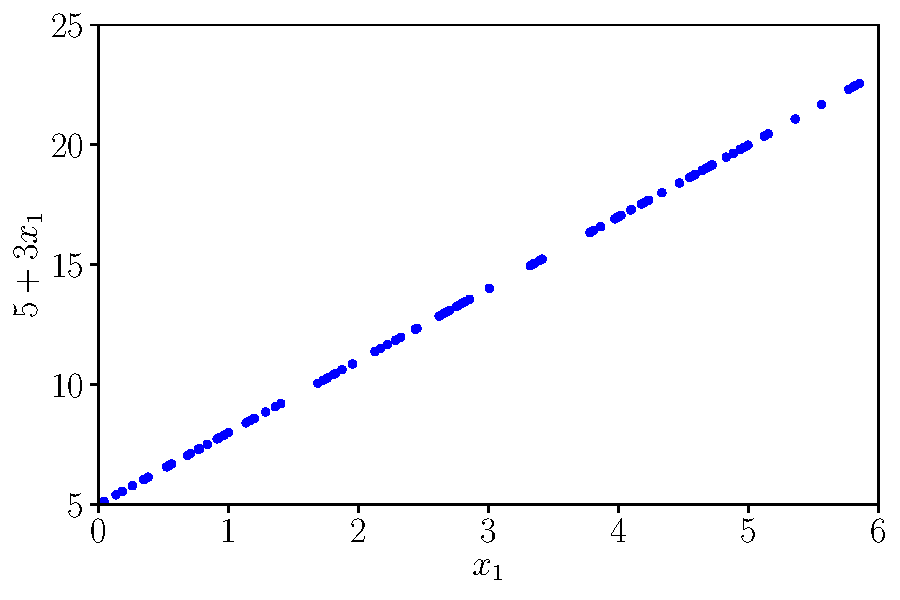
\includegraphics[width=\wMD]{einleitung/linear-data.pdf}
  \caption{Die generierten Daten}
  \label{plot:linear-data}
\end{figure}

\noindent
Die Daten sehen sehr gerade aus, damit das Problem nicht zu einfach ist
addieren auf Seiten der $y$-Werte zufälliges Rauschen:
\begin{pythoncode}
y += 3 * rng.standard_normal((100, 1))
\end{pythoncode}
Dies sollte das Problem ein wenig realistischer gestallten.
Die so modifizierten Daten sind in \autoref{plot:linear-data-noise} zu sehen.
\newpage
\begin{figure}[h!]
  \centering
  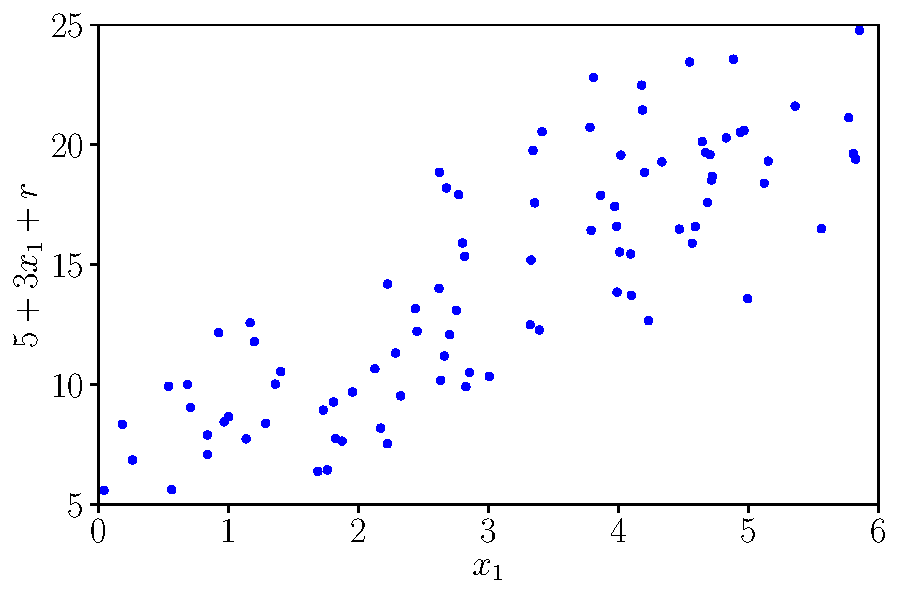
\includegraphics[width=\wMD]{einleitung/linear-data-noise.pdf}
  \caption{Die generierte Daten plus zufälliges Rauschen}
  \label{plot:linear-data-noise}
\end{figure}
\noindent
Das Regressionsproblem besitzt eine Eingabe $x_1$ und eine Ausgabe $y$.
Ein echtes Problem besteht in der Regel aus mehreren Eingaben und manchmal
aus mehreren Ausgaben. Mehrdimensionale Daten lassen sich allerdings nur schwierig
visualisieren. Ziel des Modells ist es nun eine Gerade zu finden, welche die
Daten möglichst gut beschreibt. Die Geradengleichung hat die folgende Form:
\begin{align}
  \text{1 Feature}\qquad    & \yhat = \theta_0 + \theta_1 \cdot x_1   \\
  \text{$n$ Features}\qquad & \yhat = \theta_0 + \theta_1 \cdot x_1 +
  \theta_2 \cdot x_2 + \ldots + \theta_n \cdot x_n
\end{align}
Die griechischen Buchstaben Theta $\theta_i$ beschreiben die erlernbaren Parameter und
der Funktionswert $\yhat$ (gesprochen \enquote{y-Hut}) beschreibt die Prognose.
Das Training kann in Python mit nur wenigen Zeilen Code durchgeführt werden:
\begin{pythoncode}
from sklearn.linear_model import LinearRegression
lin_reg = LinearRegression()
lin_reg.fit(x, y)
\end{pythoncode}
Wir verwenden das \pythoninline{LinearRegression} Modell von Scikit-Learn
und rufen die \pythoninline{fit} Methode zusammen
mit den Trainingsdaten und Sollwerten auf, um das Modell zu trainieren.
Die trainierten Parameter befinden sich in den Attributen \pythoninline{intercept_}
und \pythoninline{coef_}:
\begin{pyconcode}
>>> lin_reg.intercept_, lin_reg.coef_
(array([4.84609918]), array([[3.03831479]]))
\end{pyconcode}
Nicht schlecht, das Modell vermutet $\yhat = 4.85 + 3.04x_1$, wobei die ursprünglich
Funktion $y = 5 + 3x_1 + r$ war. Die genauen Werte konnten aufgrund des Rauschens
nicht wiedergewonnen werden. Die Regressionsgerade ist
in \autoref{plot:linear-data-prediction} zu sehen.
\begin{figure}[h!]
  \centering
  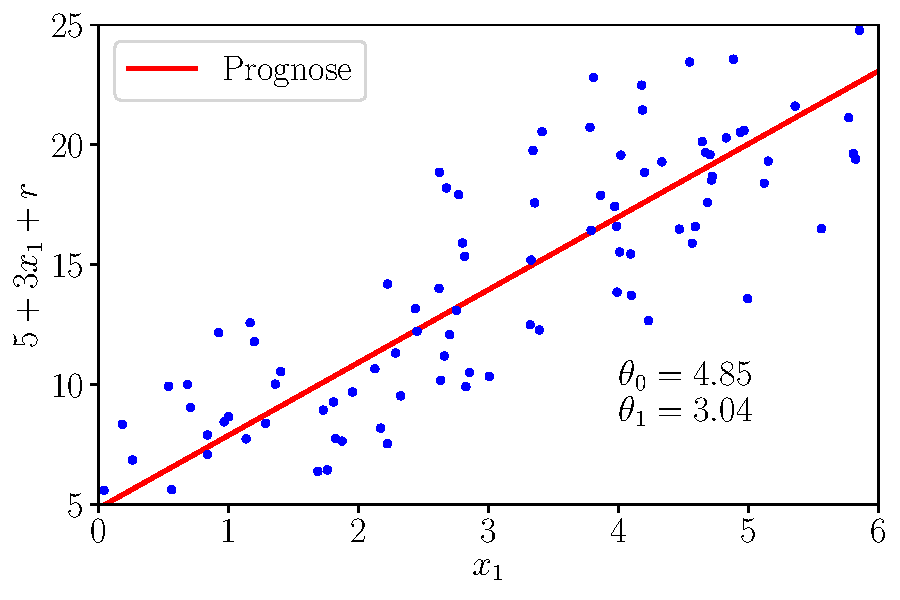
\includegraphics[width=\wMD]{einleitung/linear-data-prediction.pdf}
  \caption{Regressionsgerade}
  \label{plot:linear-data-prediction}
\end{figure}

\noindent
Der restliche Teil dieser Arbeit wird sich mit einer
speziellen Form von KI-Modellen beschäftigen: diese sind künstliche
neuronale Netze.

\section{Neuronale Netze Vergangenheit bis Heute}
Die Natur hat bereits eine unzählige Menge von Erfindungen
inspiriert, es liegt daher nahe, die Funktionsweise des Gehirns zu
untersuchen, um ein intelligentes System zu entwickeln.
Der Prozess, ein neuronales Netz zu trainieren, nennt sich Deep Learning (DL).
DL ist keine neue Idee:
Der Neurophysiologie Warren McCulloch und der Mathematiker Walter Pitts
haben das Prinzip im Jahr 1943 erstmalig öffentlich eingeführt
\parencite[280]{book:hands-on-ml}. Der frühe Erfolg von neuralen
Netzen brachte Enthusiasmus und große Erwartungen,
doch als sich in den 70er-Jahren herausstellte, dass diese Erwartungen nicht erfüllt
werden können, verlangsamte sich die Forschung und die finanziellen Fördermittel
wurden weniger \parencite[280]{book:hands-on-ml}.
Es ist nur kürzlich, dass neuronale Netze einen neuen Aufschwung erleben
und dies wahrscheinlich nicht mehr nur eine Wiederholung der Vergangenheit ist.
Die folgenden Punkte begründen diese Vermutung \parencite[280]{book:hands-on-ml}:
\begin{itemize}
  \item Durch die immer stärker digitalisierte Welt
        entstehen sehr große Mengen an Daten.
        Die Forschung und Praxis hat gezeigt, dass tiefe neuronale Netze umso besser funktionieren,
        je mehr Trainingsdaten zur Verfügung stehen. Diese steht im Gegensatz
        zu anderen Lernverfahren, wessen Leistung ab einer bestimmten
        Datenmenge typischerweise begrenzt ist.
  \item Rechenstarke CPUs und GPUs machen es möglich,
        auch große neuronale Netze
        schnell zu trainieren. Das Training eines neuronalen
        Netzes ist ein sehr iterativer Prozess.
        Es beginnt häufig mit einer Idee,
        gefolgt von der Umsetzung und anschließender Experimente, um die ursprüngliche
        Idee zu bessern.
        \begin{tikzpicture}[
    node distance=0.5,
    arr/.style={-Triangle, shorten <= 2mm, shorten >=2mm, thick}
  ]

  \node (idee) {Idee};
  \node [below right= of idee] (umsetzung) {Umsetzung};
  \node [below left= of idee] (experiment) {Experimentieren}
  (experiment) edge [arr, bend left=20] (idee)
  (idee) edge[arr, bend left=20] (umsetzung)
  (umsetzung) edge[arr, bend left=30] (experiment);
\end{tikzpicture}

        \noindent
        Dieser Ablauf ist in \autoref{fig:nn-training-process} zu sehen.
        Geht das Training schnell, kann dieser Kreislauf öfter durchlaufen
        werden und es wird ein besseres Ergebnis erzielt.
  \item Von Spracherkennung bis hin zum autonomen Fahren,
        es gibt bereits viele hervorragende Anwendungen, welche zeigen,
        wie gut Deep Learning funktioniert, um komplexe Probleme zu lösen.
\end{itemize}
Der Versuch, ein neuronales Netz von Beginn an neu aufzubauen,
würde eine Menge Arbeit in Anspruch nehmen.
Glücklicherweise können viele der komplexesten Schritte
(wie die Implementierung des Backpropagation-Algorithmus)
automatisiert werden und es gibt eine Menge von
Deep-Learning-Bibliotheken, welche diese Aufgabe übernehmen.
Die populärste Deep-Learning-Bibliothek (in Bezug auf Verweise in Forschungsarbeiten,
GitHub-Sterne, Verwendung in Firmen usw.) trägt den Namen TensorFlow
\parencite[376]{book:hands-on-ml}.
Es wurde von dem Google Brain entwickelt und ist seit November 2015
ein Open-Source-Projekt \parencite[376]{book:hands-on-ml}.
Es besitzt eine ähnliche API wie NumPy und Scikit-Learn
aus \autoref{sec:lernmethoden}, mit zusätzlicher
GPU Unterstützung und Deep Learning Fokussierung.
Die restlichen Beispiele dieser
Arbeit werden die TensorFlow Bibliothek verwenden.

\section{Deep Learning und Mobile Geräte}
\label{sec:dl-mobile}
In dieser Bachelorarbeit geht es um Maschinelles Lernen auf mobilen Geräten.
Maschinelles Lernen auf mobilen Geräten bringt einige
zusätzliche Herausforderungen mit sich.
Ein großes neuronales Netz mit vielen erlernbaren
Parametern (zum Teil im acht- bis neunstelligen Bereich) kann eine Dateigröße von
\qty{100}{\mega\byte} schnell überschreiten.
Solch ein großes Modell braucht lange, um es herunterzuladen,
verwendet viel RAM und CPU und all dies macht die Anwendung langsam,
erhitzt das Gerät und verbraucht schnell die Batterie \parencite[685]{book:hands-on-ml}.
Es wird eine Lösung benötigt, die ein Modell mobilfreundlich,
effizient und kleiner macht, ohne dabei zu viel Genauigkeit einzubüßen.
Die TensorFlow Lite Bibliothek (TFLite)
bietet verschiedene Werkzeuge an, um ein Modell auf mobilen und eingebetteten
Systemen bereitzustellen, mit den folgenden drei Zielen \parencite[685]{book:hands-on-ml}:
\begin{itemize}
  \item Reduzieren der Modellgröße für kürzere Downloadzeiten und
        geringere RAM Nutzung.
  \item Reduzieren der benötigten Rechenleistung, um eine Prognose durchzuführen,
        für weniger Verzögerung, Batterieverbrauch und Hitzeentwicklung.
  \item Anpassen des Modells an gerätespezifische Einschränkungen.
\end{itemize}
Eine genauere Beschreibung des Ablaufs und technische Details, werden
im nächsten Kapitel untersucht.
Das Gerät, welches in dieser Arbeit verwendet wird, ist der Siemens SIMATIC
IOT2050. Es ist von Aufbau und Kapazität ähnlich wie ein Raspberry Pi
und wird mit Netzteil betrieben.
Dies macht einen hohen Batterieverbrauch zu keinem entscheidenden Faktor,
jedoch sind geringe RAM Nutzung, Verzögerung und Hitzeentwicklung
noch immer sehr ausschlaggebend.
Der IOT2050 ist in \autoref{fig:iot2050} zu sehen.
\newpage
\begin{figure}[h!]
  \centering
  \begin{tikzpicture}
    [every node/.style={inner sep=0}]

    \node [] (a) {
      \begin{minipage}{0.45\textwidth}
        \includegraphics[width=1\textwidth]{einleitung/iot2050-haus.png}
        \caption*{(a)}
      \end{minipage}
    };
    \node [right= of a] (b) {
      \begin{minipage}{0.45\textwidth}
        \includegraphics[width=1\textwidth]{einleitung/iot2050.png}
        \caption*{(b)}
      \end{minipage}
    };

    \node[draw=Red, rectangle, thick, yshift=29.5mm, xshift=3.5mm,
      minimum width=2.5cm, minimum height=2.5cm] at (b.south) {};
  \end{tikzpicture}
  \caption{Siemens SIMATIC IOT2050 mit (a) und ohne (b) Gehäuse und
    Google Coral Edge TPU ML accelerator (b) als Half-Mini PCIe Karte in Rot markiert}
  \label{fig:iot2050}
\end{figure}
\noindent
Die rechte Seite der Abbildung zeigt eine weitere Hardwarekomponente:
Die Google Coral Edge TPU. Tensor Processing Units (TPUs)
sind eine von Google entwickelte anwendungsspezifische Chipfamilie
speziell dafür ausgerichtet, die Inferenzgeschwindigkeiten
von Deep-Learning-Netzen zu optimieren \parencite{online:edge-tpu}.
Da sie von Google entwickelt werden, können sie zusammen
mit TensorFlow Lite Modellen verwendet werden. Der IOT2050 benutzt
ein Debian basiertes Grundimage und enthält ein
Texas Instruments System-on-a-Chip zusammen mit einem ARM-64-Bit-Prozessor.
\footnote{Mehr hardwarespezifische Informationen befinden sich in den Datenblättern zum
  IOT2050 (\url{https://support.industry.siemens.com/cs/document/109779016/simatic-iot2050})
  und der Google Coral Mini PCIe Karte (\url{https://coral.ai/docs/mini-pcie/datasheet/}).}

\section{Beschreibung des Problems}
\label{sec:problem-description}
Zu Beginn der Arbeit stellte sich der Autor die Frage:
\enquote{Wie kann ein System entwickelt werden, mit dem verschiedene DL-Modelle
  verwaltet werden können, welches modular und einfach erweiterbar ist
  und über gemeinsame Schnittstellen im Netz kommuniziert?}
Das System soll gut zusammen mit der Idee des Internets der Dinge
(engl. Internet of Things, IoT) integriert werden können.
Die Modularität ist deshalb wichtig, da auch IoT aus vielen vernetzten
Einzelelementen besteht und das System diese Architektur widerspiegeln sollte.
Die allgemeine Struktur einer solchen Anwendung ist \autoref{fig:general-architecture} zu
sehen. 
\begin{figure}[h!]
  \centering
  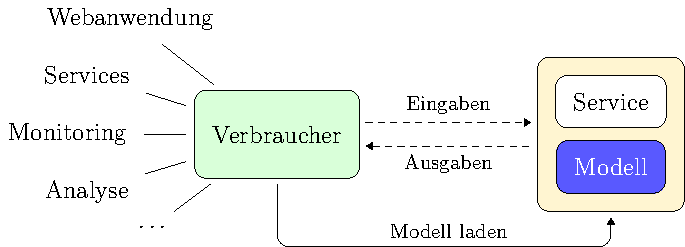
\includegraphics{einleitung/general-architecture.pdf}
  \caption{Der Aufbau einer serviceorientierten Anwendung für mobiles Maschinelles Lernen}
  \label{fig:general-architecture}
\end{figure}

\noindent
Der in Gelb markierte Service ist eine Anwendung, welche
lokal auf einem mobilen Gerät (wie dem IOT2050) ausgeführt wird.
Es verwaltet ein veröffentlichtes Modell und führt mit diesem
die Anfragen des Verbrauchers aus (\zB{} ob es sich bei einer E-Mail um Spam handelt).
Verbraucher können ganz unterschiedliche Aufgaben und Ziele haben, sie müssen
als einzige Einschränkung lediglich das verwendete Protokoll
zur Servicekommunikation verstehen.
Dies macht ein solches System sehr flexible.
Auf Verbraucherseite wird in dieser Arbeit
ein besonderer Wert auf die Umsetzung einer Webanwendung gelegt.
Die Webseite soll zeigen, wie das System verwendet
werden kann. Für einen Kunden, der daran interessiert ist, eine
KI gestützte Anwendung zusammen mit einem Gerät wie dem IOT2050
zu entwickeln, könnte diese Anwendungen als ein Demoprojekt dienen,
das zeigt, welche Möglichkeiten durch mobiles
Maschinelles Lernen und der Google Coral Edge TPU zusammen mit Siemens-Geräten
geboten werden.
Ein Ausschnitt aus der Benutzeroberfläche ist in
\autoref{fig:ui-classification-example} zu sehen.
\newpage
\begin{figure}[h!]
  \centering
  \begin{tikzpicture}
    \node [] {
      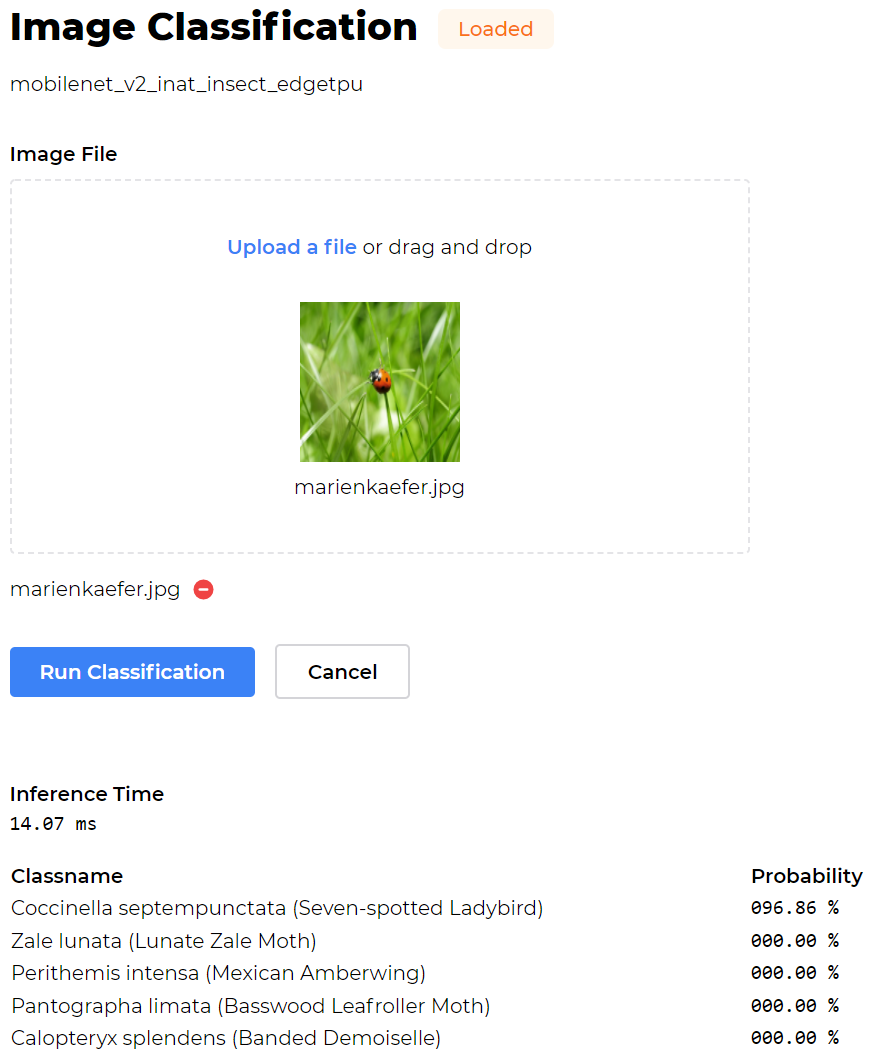
\includegraphics[width=0.75\textwidth]{einleitung/website.png}
    };
  \end{tikzpicture}
  \caption{Ausschnitt aus der Benutzeroberfläche}
  \label{fig:ui-classification-example}
\end{figure}
\noindent
Zu sehen ist der Teil der Webseite zur Klassifizierung von Bilddateien.
Das zurzeit geladene Modell ist ein für die Edge TPU kompiliertes
TFLite-Modell (basierend auf der MobileNetV2 Architektur),
welches in der Lage ist, 1000 unterschiedliche
Insektenbilder zu unterscheiden. Das ausgewählte Bild zeigt
einen Marienkäfer, weiter unten ist zu sehen, dass dieser durch das Modell mit
einer Wahrscheinlichkeit von \qty{96.86}{\percent} richtig erkannt wurde.
Die Inferenzgeschwindigkeit beträgt \qty{3.98}{\milli\second}.
Eine genauere Untersuchung der entwickelten Anwendung wird
in \autoref{chap:application} vorgenommen.
\chapter{Trainieren des ersten Neuronale Netzes}
In dem vorherigen Kapitel haben wir gesehen,
was Maschinelles Lernen bedeutet, welche
Probleme es hilft zu lösen und warum sich
Deep Learning in der heutigen Zeit mehr und mehr durchsetzt.
Es konnte außerdem das Ziel dieser Arbeit
beschrieben und einen ersten Einblick
in die verwendete Hardware gegeben werden.
In diesem Kapitel soll es darum gehen, die
TensorFlow Bibliothek kennenzulernen
und zu zeigen wie ein Deep-Learning-Modell
für mobile Geräte (und der Google Coral Edge TPU) bereitgestellt wird.
Das Kapitel ist gegliedert nach den folgenden Schritten:
\begin{enumerate}
  \item Hole den Trainingsdatensatz.
  \item Trainiere ein neuronales Netz mit TensorFlow.
  \item Bewerte die Ergebnisse des Modells.
  \item Verbessere das Modell.
  \item Konvertiere das Modell in ein mobil- und TPU-kompatibles Format.
  \item Schreibe Code, um auf dem Gerät Prognosen durchzuführen.
\end{enumerate}
Die Idee dieses Kapitels stammt aus Kapitel 4 des Buchs \citetitle{book:tiny-ml}
von \textcite{book:tiny-ml} (welche involviert in der Entwicklung
der TensorFlow Lite Bibliothek sind) mit einigen
anwendungs- und hardwarespezifischen Änderungen.

\section{Das Ziel des Modells}
Ähnlich wie \autoref{sec:lernmethoden} handelt es sich
um ein einfaches Modell mit nur einer Ein- und Ausgabe.
Die zu modellierenden Daten sind etwas komplexer,
es geht um eine bekannte trigonometrische Funktion: der Sinuskurve.
Das Ziel des Modells ist es also, durch eine Eingabe $x$
den $y$-Wert $\sin(x)$ zu bestimmen.
In einer echten Anwendung könnte
diese Zahl natürlich direkt ermittelt werden,
das Beispiel soll jedoch zeigen,
wie mit Deep Learning (und sehr kleinen Netzen)
bereits anspruchsvollere, nicht lineare Daten gut modelliert werden können.
Die Sinusfunktion ist in \autoref{plot:sine-curve} zu sehen.
\begin{figure}[h!]
  \centering
  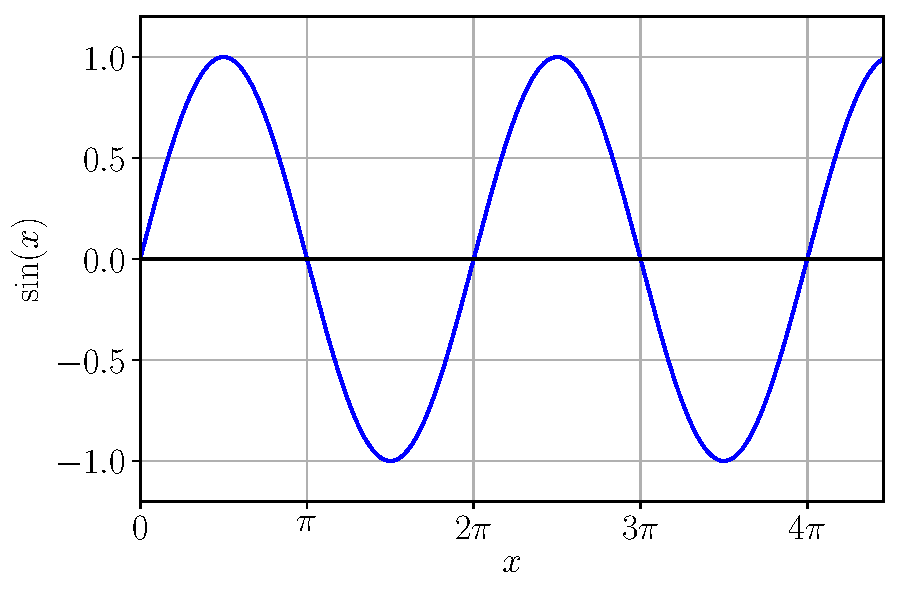
\includegraphics[width=\wMD]{first-nn/sine-curve.pdf}
  \caption{Die Sinusfunktion}
  \label{plot:sine-curve}
\end{figure}

\section{Generieren der Daten}
Neuronale Netze können komplexe Muster in den zugrundeliegenden Daten erkennen
und dabei sehr vielseitig eingesetzt werden.
In diesem Beispiel geht es wie zuvor um ein einfaches Regressionsproblem,
ein neuronales Netz kann genauso gut, aber auch für
Klassifizierung, Bildanalyse, Videoanalyse, unüberwachtes Lernen und vieles mehr verwendet werden.
Die Trainingsdaten können mit TensorFlow generiert werden und
die Vorgehensweise ist hierbei sehr ähnlich wie mit der Verwendung von NumPy:
\begin{pythoncode}
import tensorflow as tf
import math

SAMPLES = 2000

tf.random.set_seed(42)

x = tf.random.uniform((SAMPLES, 1), minval=0, maxval=2*math.pi)
tf.random.shuffle(x)

y = tf.math.sin(x)
\end{pythoncode}
Der vorhergehende Code generiert zwei Spaltenvektoren
(Trainingsdaten \pythoninline{x} und Label \pythoninline{y})
mit jeweils 2000 Werten im Bereich 0 bis $2\pi$.
Dieser Bereich nennt sich die Periode der Sinusfunktion,
da sich die Funktionswerte von dort an immer wiederholen.
Damit das Problem realistischer ist, wird auch für diese Daten
zufälliges Rauschen hinzugefügt:
\begin{pythoncode}
y += 0.25 * tf.random.normal(y.shape)
\end{pythoncode}
\begin{figure}[h!]
  \centering
  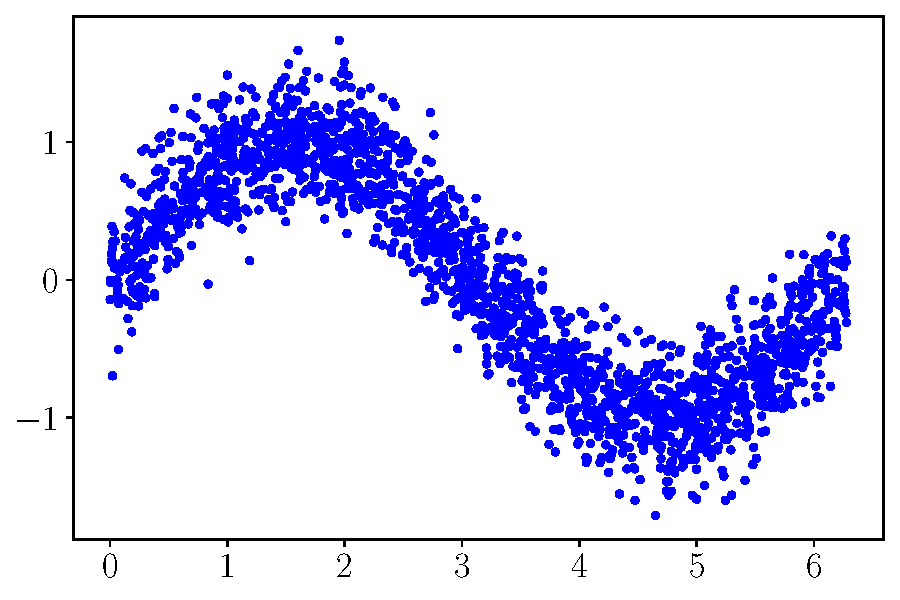
\includegraphics[width=\wMD]{first-nn/sine-data-noise.pdf}
  \caption{Die generierten Sinusdaten plus zufälliges Rauschen}
\end{figure}

\section{Aufteilen der Trainingsdaten}
\label{sec:split-train-data}
Um die Qualität eines Modells bewerten zu können, werden
mehr Daten benötigt als lediglich die Trainingsbeispiele.
Dies ist der Grund warum es für gewöhnlich mehr als nur einen
Datensatz gibt. Eine typische Vorgehensweise ist die Aufgliederung der Daten
in drei Teile: dem \textit{training}, \textit{validation} und \textit{test set}.
Die Schritte, um ein passendes Modell für ein Problem zu finden, sind die Folgenden:
\begin{enumerate}
  \item Probiere verschiedene Ideen aus und trainiere einige Modelle mithilfe des
        \textit{training set}.
  \item Bewerte die Qualität der Modelle anhand des \textit{validation set} und wähle
        einen oder mehrere der vielversprechendsten Kandidaten aus.
  \item Verbessere die Leistung der ausgewählten Modelle am \textit{validation set}
        solange, bis ein Modell mit der gewünschten Qualität gefunden wurde.
        Das ausgewählte Modell kann schließlich durch das
        \textit{test set} evaluiert werden, um den Generalisierungsfehler abzuschätzen.
\end{enumerate}
Im Training sollte der Algorithmus lediglich die Trainingsdaten
zu Gesicht bekommen. Dies hilft bekannten
Fehlerquellen wie der Überanpassung (dem Gegenstück zur Unteranpassung, engl.
\textit{overfitting} und \textit{underfitting}) vorzubeugen.
Die folgende Abbildung soll die beiden Begriffe deutlich machen:
\begin{figure}[h!]
  \centering
  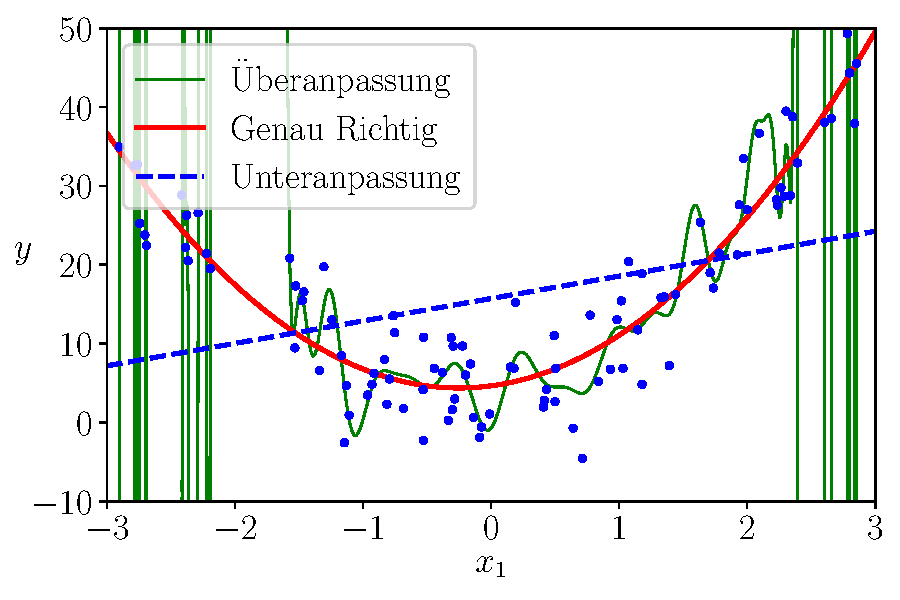
\includegraphics[width=\wLG]{first-nn/over_underfitting.pdf}
  \caption{Überanpassung und Unteranpassung am Beispiel einer
  quadratischen Funktion \parencite[131]{book:hands-on-ml}}
\end{figure}

\noindent
Modelliert ein Algorithmus die Struktur der Trainingsdaten zu gut, dann
ist die Rede von Überanpassung. Dies ist zu sehen
durch die grüne Linie. Die Funktion mit sehr vielen Features
mag die Trainingsdaten am besten beschreiben,
schafft es aber nicht auf neue Daten zu verallgemeinern.
Überanpassung kann erkannt werden, wenn die Leistung des Modells am
\textit{training set} steigt, während sie am \textit{validation set}
sinkt. Das Gegenstück der Überanpassung ist die
Unteranpassung. Dies zu sehen durch die blau gestreifte Linie.
Das Modell (mit nur linearen Features)
schafft es nicht die Trainingsdaten gut genug zu beschreiben.
Die besten Ergebnisse werden in diesem Beispiel durch die rote Linie erzeugt.
Um die zuvor generierten Trainingsdaten aufzuteilen,
kann die TensorFlow Methode \pythoninline{tf.split}
verwendet werden:
\begin{pythoncode}
# Wir verwenden 50% der Daten für training und 30% für testing.
# Die restlichen 20% werden für validation verwendet.
TRAIN_SIZE = int(0.5 * SAMPLES)
TEST_SIZE = int(0.3 * SAMPLES)
VAL_SIZE = SAMPLES - TRAIN_SIZE - TEST_SIZE

# Gliedere den Datensatz in drei Teile auf
x_train, x_test, x_val = tf.split(x, [TRAIN_SIZE, TEST_SIZE, VAL_SIZE])
y_train, y_test, y_val = tf.split(y, [TRAIN_SIZE, TEST_SIZE, VAL_SIZE])

# Verifiziere die Aufteilung, durch summieren der Größen
assert tf.size(x_train) + tf.size(x_test) + tf.size(x_val) == SAMPLES
\end{pythoncode}
Die drei Datensätze können in der folgenden Abbildung farblich dargestellt werden:
\begin{figure}[h!]
  \centering
  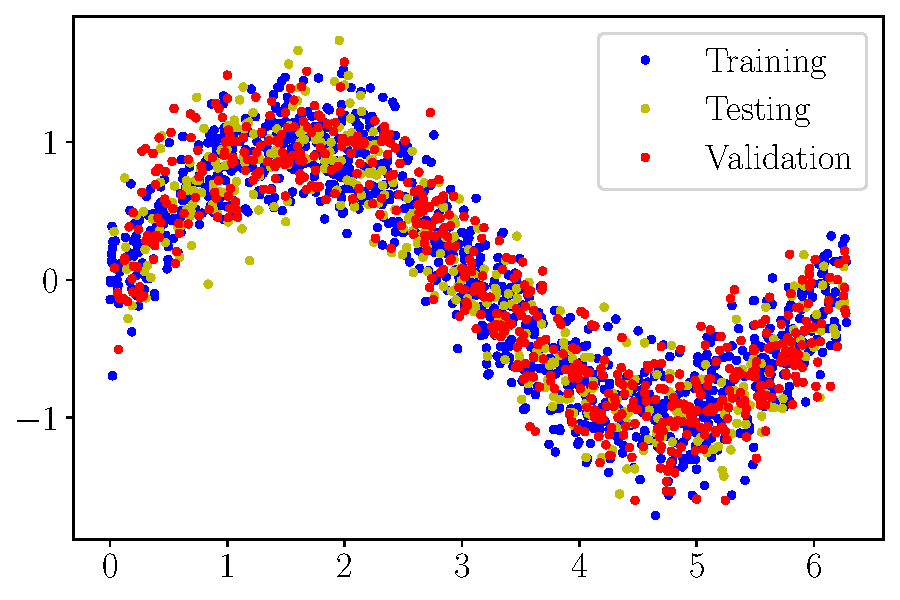
\includegraphics[width=\wMD]{first-nn/sine-data-noise-split.pdf}
  \caption{Aufteilung der Sinusdaten in
  \textit{training}, \textit{validation} und \textit{test set}}
\end{figure}

\section{Entwurf des ersten Modells}
\label{sec:modellentwurf}
Ein neuronales Netz besteht aus mehreren kleinen Einheiten (auch Neuronen genannt).
Jedes Neuron nimmt entgegen ein bis $n$ numerische Eingaben, führt einige
einfache Berechnungen durch und produziert eine numerische Ausgabe.
Alleine kann ein Neuron kaum die einfachsten Probleme lösen, doch zusammen
durch Komposition und Training haben sie das Potenzial,
die komplexe Welt verstehen.
Der Aufbau eines einzelnen Neuron ist in \autoref{fig:nn-neuron} zu sehen.
\begin{figure}[h!]
  \centering
  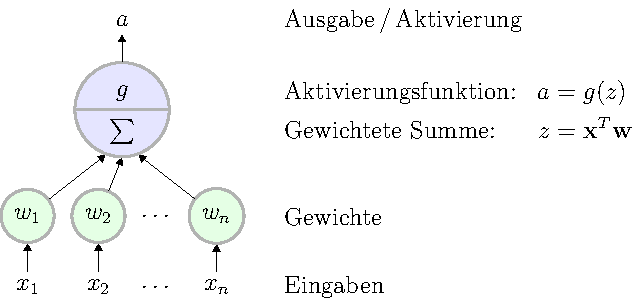
\includegraphics{first-nn/nn-neuron.pdf}
  \caption{Der Aufbau eines einzelnen Neuron}
  \label{fig:nn-neuron}
\end{figure}

\noindent
Als erster Schritt wird eine gewichtete Summe
($z = w_1x_1 + w_2x_2 +\dotsb+ w_nx_n + b = \mathbf{x}^T\mathbf{w} + b$)
der Eingabewerte plus Bias-Wert berechnet. Die Elemente $\mathbf{x}$ und $\mathbf{w}$
sind Spaltenvektoren der Form: $(x_1,\dotsc,x_n)^T$ und $(w_1,\dotsc,w_n)^T$.
\footnote{Wie immer wird versucht Berechnungen als Vektor- und Matrixoperationen
auszudrücken um CPU und GPU Beschleunigung auszunutzen.}
Der zweite Schritt wendet eine Aktivierungsfunktion auf diese Summe an und dies
erzeugt die Ausgabe: $a = g(z)$. Die Ausgabe eines Neurons
wird typischerweise die Aktivierung genannt. Ein neuronales Netz
besteht aus der Komposition verschiedener Neuronen und die
Gewichte und Bias-Werte stellen die erlernbaren Parameter dar.
\begin{figure}[h!]
  \centering
  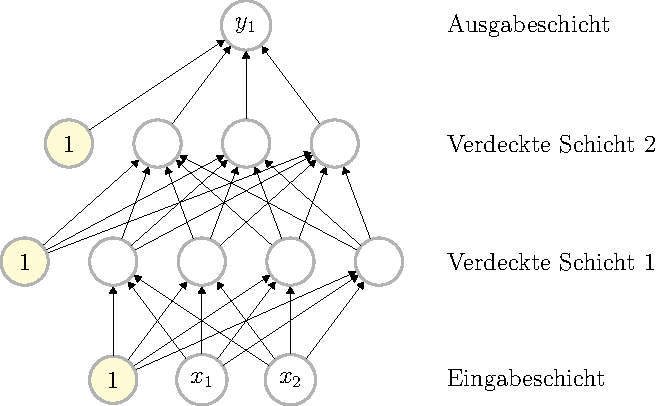
\includegraphics{first-nn/example-nn.pdf}
  \caption{Ein einfaches neuronales Netz mit zwei verdeckten Schichten}
  \label{fig:example-nn}
\end{figure}
\noindent
\autoref{fig:example-nn} zeigt ein einfaches neuronales Netz
mit zwei verdeckten Schichten (engl. \textit{hidden layers}),
zwei Eingaben und einer Ausgabe.
Verdeckte Schichten sind all diejenigen Schichten, die nicht Ein- oder Ausgabe sind.
Jede Schicht außer der Ausgabeschicht enthält ein Bias-Neuron
(in Gelb markiert), welches immer Eins ausgibt, aber auch trainiert werden kann
und ist vollständig mit der nächsten Schicht verbunden.
Ein neuronales Netz wird tief genannt, wenn es viele verdeckte Schichten besitzt.
\footnote{In den 1990er-Jahren wurde ein neuronales Netz
mit mehr als zwei verdeckten Schichten als tief angesehen.
Da es aber heutzutage Netze mit Dutzend und Hunderten von Schichten
gibt, ist die Definition von \enquote{tief} etwas schwammig \parencite[289]{book:hands-on-ml}.}
Es wird durch einen Algorithmus trainiert, der
sich Backpropagation nennt.
Backpropagation ist der weitaus mathematischste Teil von
Deep Learning, da der Schwerpunkt dieser Arbeit auf der Entwicklung einer
Anwendung liegt, werden wir nicht im Detail untersuchen,
wie dieser und verwandte Algorithmen wie das Gradientenabstiegsverfahren
funktionieren. Zusätzlich können diese Methoden durch Deep-Learning-Bibliotheken
wie TensorFlow automatisiert werden. Es wird jedoch versucht, einige
Intuitionen zu geben.\\[8pt]
Kurzum \parencite[290-291]{book:hands-on-ml}:
Backpropagation besteht aus zwei Phasen: einem Vorwärtsdurchlauf
und einem Rückwärtsdurchlauf. Die Daten werden stapelweise verarbeitet
(\zB{} 32 Datensätze auf ein­mal) und der gesamte Trainingsdatensatz
wird mehrfach durchlaufen. Ein Trainingsdurchlauf nennt sich Epoche.\\[4pt]
Jeder Datenstapel wird an die erste Schicht des neuronalen Netzes
übergeben. Von dort wird im Vorwärtsdurchlauf die Aktivierung aller
Neuronen bis hin zur Ausgabeschicht ermittelt und die Zwischenerbnisse gespeichert.\\[4pt]
Nachdem die Ausgaben der letzten Schicht bekannt sind, kann
durch Vergleich der Sollwerte der Fehler des Netzes ermittelt werden.
Dies geschieht durch eine Kostenfunktion $J$. Im Fall eines Regressionsproblems
wird typischerweise die mittlere quadratische Abweichung verwendet
(engl. \textit{mean squared error}) \parencite[113-114]{book:hands-on-ml}:
\begin{equation}
  J(\mathbf{\hat{y}}, \mathbf{y}) =
  MSE(\mathbf{\hat{y}}, \mathbf{y}) =
    \frac{1}{m} \sum_{i=1}^{m} (\mathbf{\hat{y}}^{(i)} - \mathbf{y}^{(i)})^2
  \label{eq:mse}
\end{equation}
Die Elemente $\mathbf{\hat{y}}$ und $\mathbf{y}$ sind Spaltenvektoren
mit den Ausgaben des Netzes und den tatsächlichen Werten, die Zahl $m$
ist die Größe des Vektors, welche in diesem Fall gleich der Stapelgröße
(engl. \textit{batch size}) ist. Der Index $\mathbf{v}^{(i)}$ ist keine Potenz,
sondern beschreibt den i-ten Wert im Vektor $\mathbf{v}$.\\[4pt]
Der Rückwärtsdurchlauf im letzten Schritt ist der eigentliche Teil,
mit dem das Netz
trainiert wird. Der Algorithmus misst, wie stark jedes Gewicht den Fehler der
vorherigen Schicht beeinflusst hat und versucht, diese so anzupassen,
damit die Kostenfunktion minimiert wird.\\[8pt]
TensorFlow und insbesondere die TensorFlow Keras API
macht es einfach, neuronale Netze zu entwerfen und zu trainieren.
Keras ist eine High-Level Deep Learning API, welche
von François Chollet als Teil eines Forschungsprojekts entwickelt
wurde und seit März 2015 ein Open-Source-Projekt ist
\parencite[295]{book:hands-on-ml}. Keras kann
unabhängig von TensorFlow verwendet werden, es benötigt
jedoch eine Berechnungsgrundlage (wie TensorFlow und Co.),
mit dem die für DL erforderlichen rechenintensiven Operationen durchgeführt werden können.
In dieser Arbeit wird daher ausschließlich die \pythoninline{tf.keras} API
verwendet. Ein Modell mit Keras zu entwerfen ist unkompliziert:
\begin{pythoncode}
from tensorflow import keras

input_layer = keras.layers.Input(shape=[1])
hidden1 = keras.layers.Dense(units=16, activation="relu")(input_layer)
output_layer = keras.layers.Dense(units=1, name="output")(hidden1)

model = keras.Model(inputs=input_layer, outputs=output_layer)
\end{pythoncode}
\begin{itemize}
  \item Die erste Zeile importiert das Keras Modul von TensorFlow.
  \item Als nächstes wird die Eingabeschicht des Netzes definiert.
        Diese dient ausschließlich dazu, die Dimension der Eingabewerte festzulegen.
        Da das Modell nur eine einzige Zahl entgegen nimmt,
        ist die Dimension des Eingabevektors eins.
  \item Die nächste Zeile definiert die erste und einzige verborgene Schicht mit
        16 Neuronen (\textit{units}). Die Neuronen verwenden die ReLU
        (\textit{Rectified Linear Unit}) Aktivierungsfunktion, welche wie folgt
        definiert ist:
        \begin{equation}
          g(z) = ReLU(z) = \max(0, z)
        \end{equation}
        ReLU ist eine sehr beliebte Aktivierungsfunktion, die sich nicht
        nur einfach berechnen lässt, sondern auch in der Praxis bewährt hat
        und daher gut als Standardauswahl eignet. Es gibt viele
        weitere Aktivierungsfunktion, welche häufig eingesetzt werden.
        Vier der gewöhnlichsten sind in \autoref{fig:activation-functions}
        zu sehen.
        \begin{figure}[h!]
          \centering
          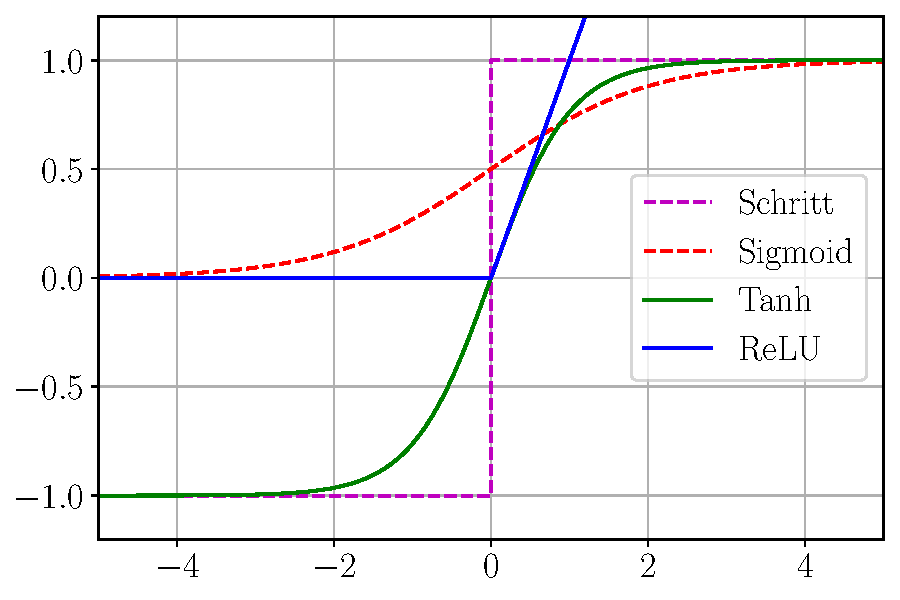
\includegraphics[width=\wMD]{first-nn/activation-functions.pdf}
          \caption{Verschiedene Aktivierungsfunktionen \parencite[292]{book:hands-on-ml}}
          \label{fig:activation-functions}
        \end{figure}
  \item Die letzten beiden Zeilen definieren die Ausgabeschicht und das endgültige
        Modell. Da das Ziel ist, einen einzigen Wert zu bestimmen, besitzt die letzte
        Ebene lediglich eine Einheit. Es wird keine Aktivierungsfunktion angegeben,
        was bedeutet, dass die Identitätsfunktion verwendet wird:
        \begin{equation}
          g(z) = z
        \end{equation}
\end{itemize}
Die \pythoninline{model.summary()} Funktion liefert einige nützliche Informationen
über das erstellte Netz, wie die verschiedenen Schichten, die Dimension
der Aktivierungen (\pyconinline{None} bedeutet eine beliebige Stapelgröße)
und die Anzahl der Parameter:
\begin{pyconcode}
>>> model.summary()
Model: "model"
_________________________________________________________________
Layer (type)                 Output Shape              Param #   
=================================================================
input_1 (InputLayer)         [(None, 1)]               0         
_________________________________________________________________
dense (Dense)                (None, 16)                32        
_________________________________________________________________
output (Dense)               (None, 1)                 17        
=================================================================
Total params: 49
Trainable params: 49
Non-trainable params: 0
_________________________________________________________________
\end{pyconcode}
Die erste verdeckte Schicht mit einer Eingabe und 16 Ausgaben besitzt
32 Parameter, 16 Gewichte ($\#Eingaben \cdot \#Ausgaben$) und 16 Bias-Werte ($\#Ausgaben$).
Die Ausgabeschicht mit 16 Eingaben und einer Ausgabe, besitzt
17 Parameter, 16 Gewichte und ein Bias-Wert.
Auf die einzelnen Schichten kann per Index oder Name zugegriffen werden:
\begin{pyconcode}
>>> model.layers
[<tensorflow.python.keras.engine.input_layer.InputLayer at 0x225b4ca4310>,
 <tensorflow.python.keras.layers.core.Dense at 0x225b4cb96d0>,
 <tensorflow.python.keras.layers.core.Dense at 0x227629dea30>]
>>> hidden1 = model.layers[1]
>>> hidden1.name
dense
>>> model.get_layer("dense") is hidden1
True
\end{pyconcode}
Die Parameter einer Schicht können ebenfalls untersucht werden,
hierfür gibt es Funktionen wie
\pythoninline{get_weights()} und \pythoninline{set_weights()}:
\begin{pyconcode}
>>> weights, biases = hidden1.get_weights()
>>> weights
array([[ 0.5445634 , -0.5741172 , -0.2190957 , -0.40382388,  0.25530386,
         0.34373027, -0.45763797, -0.1983017 , -0.3434852 ,  0.14649397,
         0.57805157, -0.4487671 , -0.34861064,  0.44097137, -0.5695514 ,
        -0.33477765]], dtype=float32)
>>> weights.shape
(1, 16)
>>> biases
array([0., 0., 0., 0., 0., 0., 0., 0., 0., 0., 0., 0., 0., 0., 0., 0.],
      dtype=float32)
>>> biases.shape
(16,)
\end{pyconcode}
Es ist zu sehen, dass die Gewichte der Ebene zufällig initialisiert wurden.
Dies ist wichtig, um die Symmetrie der Verbindungen zu brechen,
da sonst der Backpropagation-Algorithmus alle Gewichte gleichbehandeln würde
und das Training ineffektiv ist \parencite[291]{book:hands-on-ml}.
Für die Bias-Werte ist es in Ordnung, mit null zu initialisieren.
Nachdem das Modell erstellt wurde, kann die \pythoninline{model.compile()}
Methode aufgerufen werden, um die Kostenfunktion und den
Optimierungsalgorithmus festzulegen.
Als alternatives drittes Argument kann eine Liste von
zusätzlichen Messwerten angegeben werden:
\begin{pythoncode}
sgd = keras.optimizers.SGD()
model.compile(optimizer=sgd, loss="mse", metrics=["mae"])
\end{pythoncode}
Als Kostenfunktion wird die mittlere quadratische Abweichung verwendet
\eqref{eq:mse} und der Optimierungsalgorithmus ist
\textit{stochastic gradient descent} (SGD). \textit{Gradient descent}
(dt. Gradientenabstieg) ist ein allgemeiner Optimierungsalgorithmus
um eine Kostenfunktion zu minimieren \parencite[118]{book:hands-on-ml}.
Es soll in dieser Arbeit nicht im Detail untersucht werden, wie dieser
Algorithmus funktioniert, nichtsdestotrotz sind einige Intuitionen
in \autoref{appx:gradient-descent} gegeben.
Als zusätzlicher Messwert wird die mittlere absolute Abweichung
(engl. \textit{mean absolute error}) angegeben.
Die Gleichung ist sehr ähnlich wie die des $MSE$ nur das der absolute Fehler
anstelle des quadratischen Fehlers gemessen wird:
\begin{equation}
  J(\mathbf{\hat{y}}, \mathbf{y}) =
  MAE(\mathbf{\hat{y}}, \mathbf{y}) =
    \frac{1}{m} \sum_{i=1}^{m} \vert\mathbf{\hat{y}}^{(i)} - \mathbf{y}^{(i)}\vert
  \label{eq:mae}
\end{equation}
Die mittlere absolute Abweichung ist vor allem für ein Regressionsproblem
ein gutes Maß, um abzuschätzen, wie stark Prognosen im Training von
den Sollwerten abweichen.

\section{Das Modell trainieren und bewerten}
\label{sec:train-evaluate-model}
Das Netz ist nun bereit um trainiert zu werden.
Dies funktioniert den Aufruf der \pythoninline{fit} Methode:
\begin{pyconcode}
>>> EPOCHS = 300
>>> BATCH_SIZE = 16
>>> history = model.fit(x_train, y_train, epochs=EPOCHS,
...                     batch_size=BATCH_SIZE, validation_data=(x_val, y_val))
...
Epoch 1/300
63/63 [======] - 2s 4ms/step - loss: 0.5319     - mae: 0.6028
                             - val_loss: 0.3661 - val_mae: 0.5134
Epoch 2/300
63/63 [======] - 0s 3ms/step - loss: 0.3422     - mae: 0.4941
                             - val_loss: 0.2898 - val_mae: 0.4533
[...]
Epoch 300/300
63/63 [======] - 0s 3ms/step - loss: 0.2138     - mae: 0.3667
                             - val_loss: 0.2135 - val_mae: 0.3671
\end{pyconcode}
Wir übergeben das \textit{training set}, legen die Epochenzahl fest
und geben eine Stapelgröße an.
Als optionales Argument wird außerdem das \textit{validation set}
übergeben. Die Stapelgröße zeigt, wie viele Trainingsdaten betrachten werden,
bevor die Kostenfunktion bestimmt und die Gewichte und Bias-Werte
des Netzes einmal angepasst werden
(wie häufig ein Schritt des Gradientenabstiegs durchgeführt wird).
In \autoref{sec:split-train-data} wurden \qty{50}{\percent} der Daten
als \textit{training set} verwendet:
\begin{pyconcode}
>>> x_train.shape # 2000 * 50% = 1000
TensorShape([1000, 1])
\end{pyconcode}
Wie in der oberen Ausgabe zu sehen ist, macht dies
pro Epoche 63 ($1000 / 16 = \num{62.5}$) Gewichts- und Bias-Aktualisierungen.
Durch erneutes Betrachten der Parameter nach dem Training
können die Veränderungen beobachtet werden:
\begin{pyconcode}
>>> hidden1 = model.get_layer("dense")
>>> weights, biases = hidden1.get_weights()
>>> weights
array([[ 0.48667157, -0.5741172 , -0.2190957 , -0.40382388,  0.43343386,
         0.23612383, -0.45763797, -0.1983017 , -0.3434852 ,  0.7860139 ,
         0.55660063, -0.4487671 , -0.34861064,  0.41839647, -0.5695514 ,
        -0.33477765]], dtype=float32)
>>> biases
array([-0.6504982 ,  0.        ,  0.        ,  0.        , -0.5743109 ,
       -0.00350828,  0.        ,  0.        ,  0.        , -0.9752765 ,
       -0.00748946,  0.        ,  0.        , -0.00579908,  0.        ,
        0.        ], dtype=float32)
\end{pyconcode}
Nicht alle Parameter der verdeckten Schicht wurden angepasst, einige
Änderungen an den Bias-Werten sind jedoch gut zu erkennen.
Die Keras Ausgabe enthält weitere nützliche Informationen:
\begin{description}[font=\normalfont, style=nextline]
\item[\pyconinline{loss} und \pyconinline{val_loss}]
Die Ausgabe der Kostenfunktion für das \textit{training} und \textit{validation set}.
Es ist zu sehen das der Fehler während dem Training für beide Datensätze abnimmt,
was ein gutes Zeichen ist.
\item[\pyconinline{mae} und \pyconinline{val_mae}]
Die mittlere absolute Abweichung. Wie auch die Kostenfunktion
nimmt diese für beide Datensätze während dem Training ab.
Ein absoluter Fehler von \num{0.3667}
nach 300 Epochen ist allerdings noch immer relativ hoch.
Angesichts der Tatsache, dass mögliche Werte ungefähr im
Bereich $[-1, 1]$ liegen.
Dies könnte bedeuten, dass es das Netz nicht geschafft hat, die Daten
gut zu modellieren. Mehr Einblick kann gegeben werden, sobald
das Modell getestet und die Ergebnisse grafisch dargestellt werden.
\end{description}

\subsection{Grafische Darstellung des Trainings}
Die \pythoninline{fit} Methode gibt ein \pythoninline{History} Objekt zurück.
Ihr \pythoninline{History.history} Attribut
ist eine Aufzeichnung aller Messwerte in aufeinanderfolgenden Epochen:
\begin{pyconcode}
>>> history.history.keys()
dict_keys(["loss", "mae", "val_loss", "val_mae"])
>>> mse = history.history["loss"]
>>> val_mse = history.history["val_loss"]
>>> mae = history.history["mae"]
>>> val_mae = history.history["val_mae"]
>>> len(mse) == len(val_mse) == len(mae) == len(val_mae) == EPOCHS
True
\end{pyconcode}
Diese Aufzeichnungen können verwendet werden um die Trainingswerte
in Bezug auf die Epochenzahl darzustellen:
\begin{pythoncode}
import matplotlib.pyplot as plt

epochs = tf.range(0.0, EPOCHS)

fig, (ax1, ax2) = plt.subplots(2, 1, figsize=[6.4, 8])

# Stelle den MSE für beide Datensätze dar
ax1.plot(epochs, mse, "b-", label="Training")
ax1.plot(epochs, val_mse, "g-", label="Validation")

# Stelle den MAE für beide Datensätze dar
ax2.plot(epochs, mae, "b-", label="Training")
ax2.plot(epochs, val_mae, "g-", label="Validation")

[...] # Achsenbeschriftung, Gitter und Legende

plt.show()
\end{pythoncode}
\begin{figure}[h!]
  \centering
  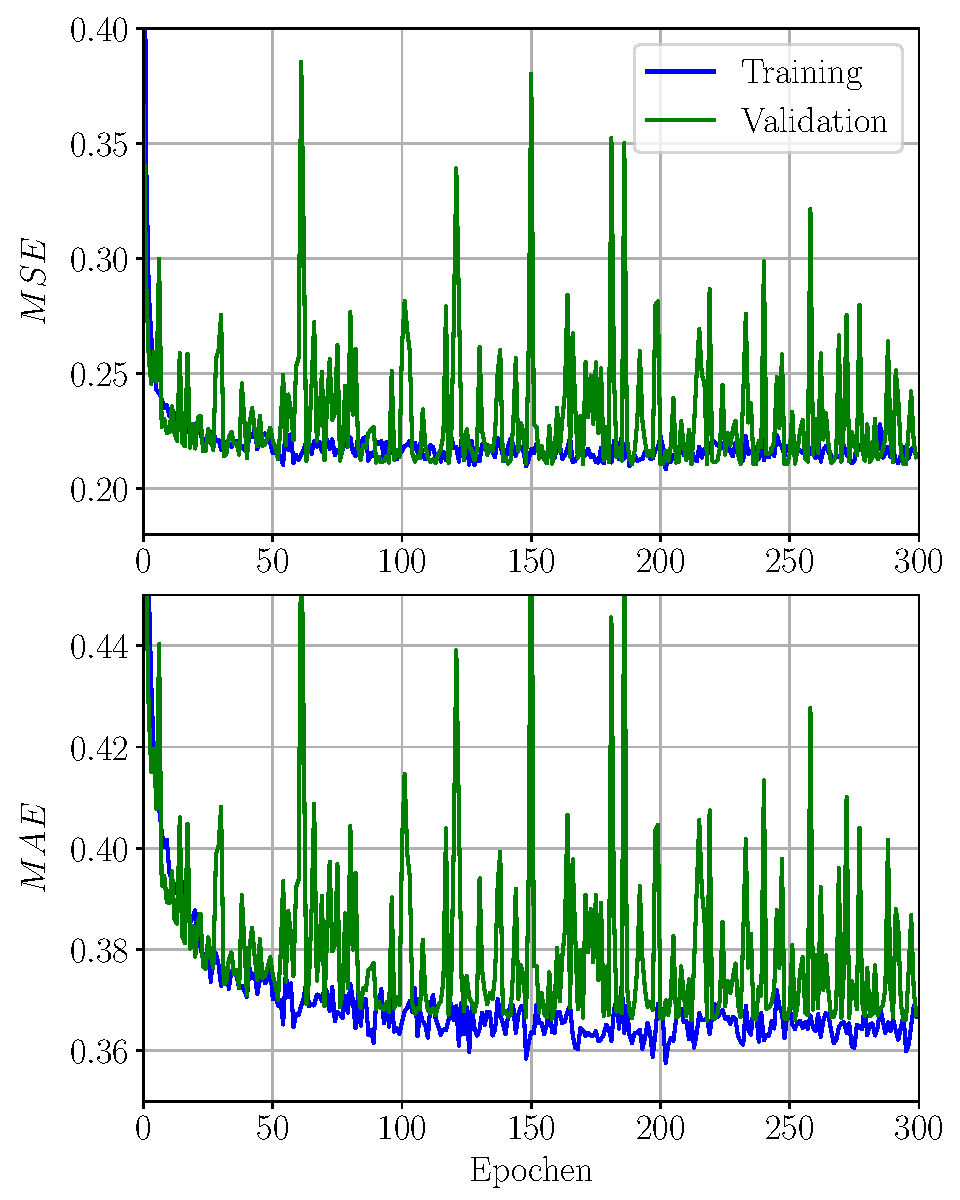
\includegraphics[width=\wMD]{first-nn/1-metrics.pdf}
  \caption{Trainingskurven: Der durchschnittliche \textit{training}
  $MSE$ und $MAE$ gemessen während jeder Epoche
  und der \textit{validation} $MSE$ und $MAE$
  gemessen am Ende jeder Epoche}
\end{figure}
\noindent
Es ist zu sehen, dass beide Fehler sowohl für das
\textit{training set} als auch das \textit{validation set}
zu Beginn des Trainings stark fallen.
Die Werte sind relativ nahe beieinander, wobei die Validierungsfehler
teilweise stark variieren, aber auf keine Überanpassung hin deuten.
Das Modell scheint nach etwa 100 bis 150 Epochen für beide Graphen
keinen großen Fortschritt mehr zu machen, weshalb
das Training bereits frühzeitig beendet werden könnte.
Der Fehler auf dem \textit{validation set} wird
am Ende jeder Epoche gemessen, während der Trainingsfehler als Durchschnittswert
während der Epoche bestimmt wird \parencite[305]{book:hands-on-ml}.
Dies ist der Grund, warum der Validierungsfehler
vereinzelt kleiner als der Trainingsfehler ist, was ungewöhnlich sein sollte:
Das Modell wurde zum Zeitpunkt der Berechnung ein wenig länger trainiert.

\subsection{Grafische Darstellung der Prognosen}
Um die Qualität des Modells weiter zu beurteilen, können einige
Prognosen mit dem \textit{training} oder \textit{validation set}
durchgeführt und die Ergebnisse angezeigt werden:
\begin{pythoncode}
predictions = model.predict(x_val)

# Zeige die Prognosen zusammen mit den Sollwerten an
plt.plot(x_val, y_val, "b.", label="Validierungsdaten")
plt.plot(x_val, predictions, "y.", label="Prognose")
[...] # Legende und die Daten der Sinuskurve
plt.show()
\end{pythoncode}
\begin{figure}[h!]
  \centering
  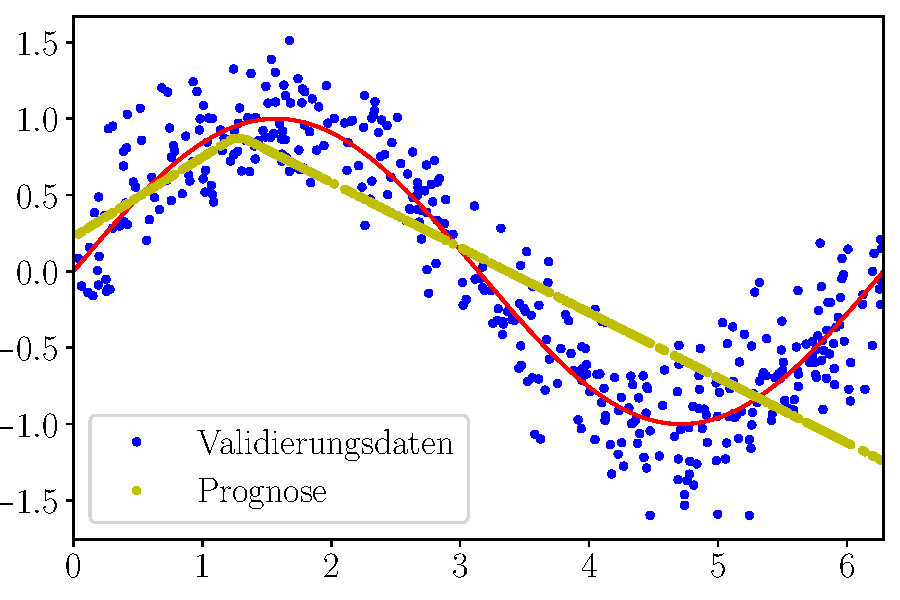
\includegraphics[width=\wMD]{first-nn/1-predictions_val.pdf}
  \caption{Ein Graph der Prognosen des Modells gegenüber der Sollwerte aus dem
  \textit{validation set} zusammen mit der Sinuskurve als Referenz}
  \label{fig:sine-underfitting}
\end{figure}
Oje, \autoref{fig:sine-underfitting} macht die zuvor gestellte Vermutung klar.
Das Modell hat es nur in einer sehr beschränkten Weise
geschafft, die Sinuskurve zu ap­pro­xi­mie­ren.
Es ist also Zeit, zurück ans Zeichenbrett zu gehen und
das Modell anzupassen, um die Qualität am \textit{validation set}
zu verbessern.

\section{Das Modell verbessern}
Es scheint, als wäre das zuvor entworfene Modell nicht mächtig genug,
um die Daten ausreichend gut zu beschreiben.
Um dieser Unteranpassung vorzubeugen, muss die Komplexität des Netzes
erhöht werden. Hierfür gibt es zwei Möglichkeiten:
Hinzufügen weiterer Schichten oder Erhöhen der Neuronenanzahl.
Das Netz soll durch zwei zusätzliche Schichten erweitert werden:
\begin{pythoncode}
input_layer = keras.Input(shape=[1])
# Erste neue Schicht mit 8 Einheiten
hidden1 = keras.layers.Dense(units=8, activation="relu")(input_layer)
# Alte Schicht mit 16 Einheiten
hidden2 = keras.layers.Dense(units=16, activation="relu")(hidden1)
# Zweite neue Schicht mit 32 Einheiten
hidden3 = keras.layers.Dense(units=32, activation="relu")(hidden2)
output_layer = keras.layers.Dense(1, name="output")(hidden3)

model = keras.Model(inputs=input_layer, outputs=output_layer)
\end{pythoncode}
Die Übersicht gibt Auskunft über die Anzahl der Parameter:
\begin{pyconcode}
>>> model.summary()
Model: "model"
_________________________________________________________________
Layer (type)                 Output Shape              Param #   
=================================================================
input_1 (InputLayer)         [(None, 1)]               0         
_________________________________________________________________
dense (Dense)                (None, 8)                 16        
_________________________________________________________________
dense_1 (Dense)              (None, 16)                144       
_________________________________________________________________
dense_2 (Dense)              (None, 32)                544       
_________________________________________________________________
output (Dense)               (None, 1)                 33        
=================================================================
Total params: 737
Trainable params: 737
Non-trainable params: 0
_________________________________________________________________
\end{pyconcode}
737 im Vergleich zu den 49 Parametern des alten Modells.
Dies sollte dem Netz sehr viel mehr Spielraum gegeben,
die Daten gut zu beschreiben.
Das Training funktioniert in gleicherweise wie zuvor:
\begin{pyconcode}
>>> sgd = keras.optimizers.SGD()
>>> model.compile(optimizer=sgd, loss="mse", metrics=["mae"])
>>> history = model.fit(x_train, y_train, epochs=EPOCHS,
...                     batch_size=BATCH_SIZE, validation_data=(x_val, y_val))
...
Epoch 1/300
63/63 [======] - 0s 4ms/step - loss: 0.4988     - mae: 0.6041
                             - val_loss: 0.3944 - val_mae: 0.5356
[...]
Epoch 300/300
63/63 [======] - 0s 4ms/step - loss: 0.0646     - mae: 0.2027
                             - val_loss: 0.0710 - val_mae: 0.2125
\end{pyconcode}
Auch die Trainingskurven können nach demselben Prinzip
generiert werden:
\begin{figure}[h!]
  \centering
  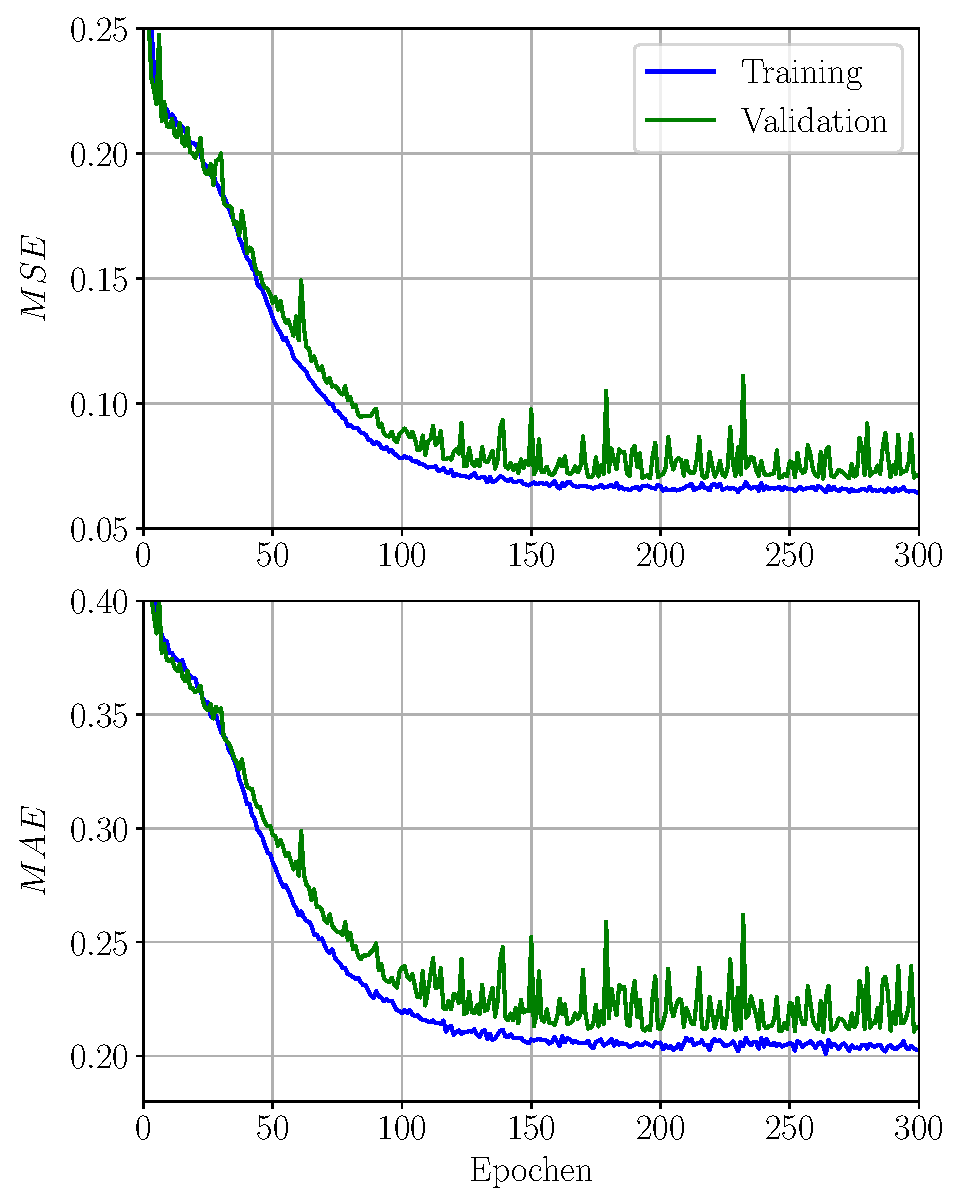
\includegraphics[width=\wMD]{first-nn/2-metrics.pdf}
  \caption{Trainingskurven des angepassten Modells}
\end{figure}

\noindent
Die Trainingsergebnisse sind vielsprechend, sowohl MSE als auch MAE
sind um einiges niedriger als zuvor und die Trainingskurven
sehen allgemein stabiler aus mit weniger großen Ausreißern.
Die grafische Darstellung der Prognosen bestätigt dieses Ergebnis:
\begin{figure}[h!]
  \centering
  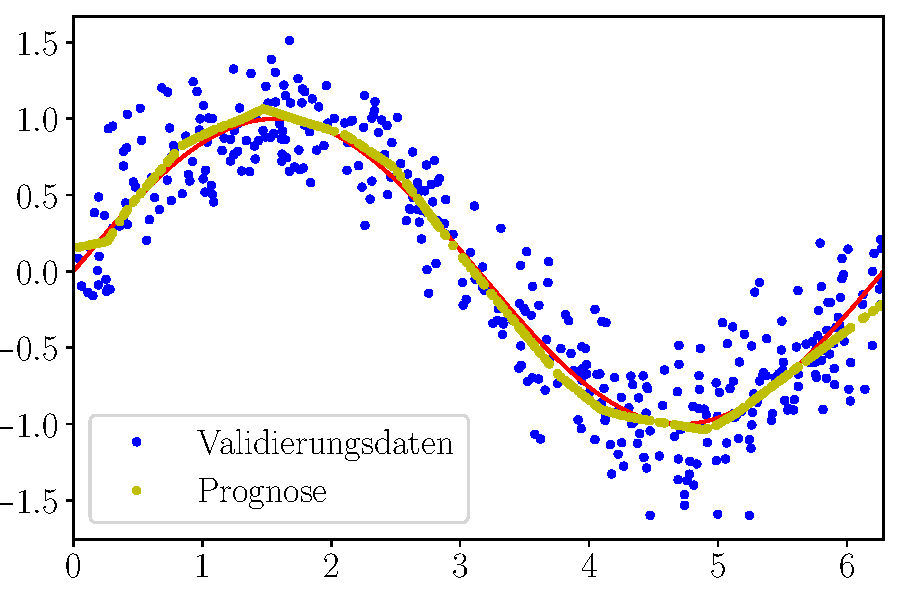
\includegraphics[width=\wMD]{first-nn/2-predictions_val.pdf}
  \caption{Ein Graph der Prognosen des verbesserten Modells gegenüber der Sollwerte aus dem
  \textit{validation set} zusammen mit der Sinuskurve als Referenz}
\end{figure}

\noindent
Das Netz scheint die Daten trotz Rauschen gut beschreiben zu können.
Die Kurve ist nicht vollständig glatt, was eine leichte Überanpassung der Trainingsdaten
indiziert. Möchte das Modell weiter verbessert werden,
könnte das Training regularisiert,
mehr Trainingsdaten gesammelt oder Rauschen beseitigt werden
(vgl. Verhinderung von Überanpassung, \cite[28]{book:hands-on-ml}).
Ist die Leistung des Modells am \textit{validation set} zufriedenstellend,
kann in den letzten Schritt übergegangen werden: Die Evaluierung am \textit{test set}.
Keras bietet hierfür die Methode \pythoninline{evaluate} an:
\begin{pyconcode}
>>> model.evaluate(x_test, y_test)
19/19 [======] - 0s 2ms/step - loss: 0.0706 - mae: 0.2078
[0.07061798125505447, 0.20783697068691254]
\end{pyconcode}
Sowohl die Werte des $MSE$ (\num{0.0706} zu \num{0.0646}) als auch
die des $MAE$ (\num{0.2078} zu \num{0.2027}) sind sehr ähnlich
wie die aus dem Training. Das Netz schafft es also auch für
bislang ungesehene Daten gute Schlüsse ziehen.
Es ist wichtig, der Versuchung zu widerstehen, das Modell nach
der Evaluierung am \textit{test set} weiter anzupassen, da die Abschätzung
des Generalisierungsfehlers ansonsten zu optimistisch wäre
\parencite[80]{book:hands-on-ml}.
Für eine endgültige Bestätigung können auch die Vorhersagen
der Testdaten ein letztes Mal grafisch dargestellt werden:
\begin{pythoncode}
predictions = model.predict(x_test)
[...] # Wie zuvor
\end{pythoncode}
\begin{figure}[h!]
  \centering
  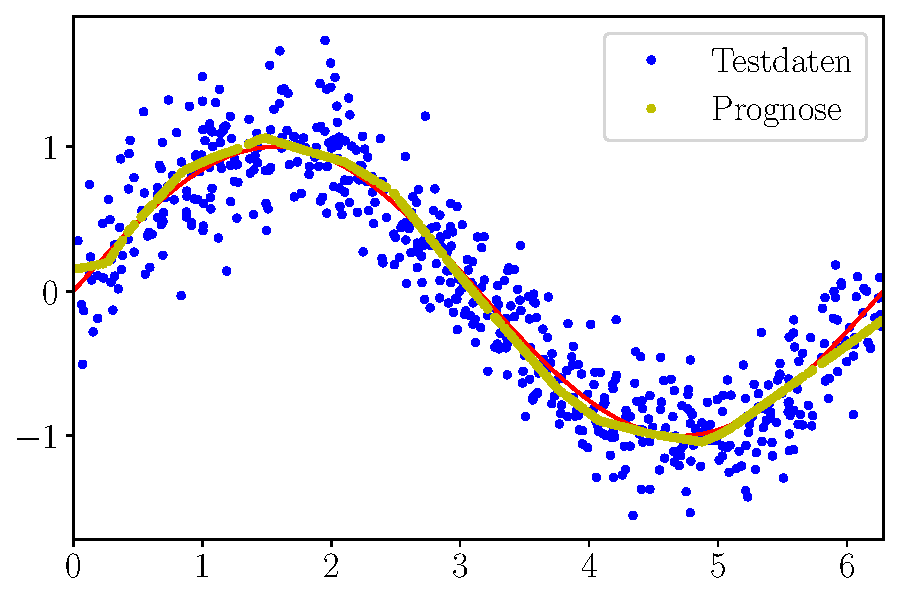
\includegraphics[width=\wMD]{first-nn/2-predictions.pdf}
  \caption{Ein Graph der Prognosen des verbesserten Modells gegenüber der Sollwerte aus dem
  \textit{test set} zusammen mit der Sinuskurve als Referenz}
  \label{fig:predictions-train-set}
\end{figure}

\section{Konvertieren des Modells nach TensorFlow Lite}
\label{sec:convert-model}
Jetzt, wo ein Modell mit der gewünschten Qualität trainiert
wurde, ist es Zeit, dieses zu veröffentlichen.
Das Modell soll für die Verwendung auf mobilen Geräten optimiert werden
und kompatibel mit Google Edge TPUs sein.
Hierfür wird Gebrauch von der TensorFlow Lite (TFLite) Bibliothek gemacht.
Wie in \autoref{sec:dl-mobile} untersucht,
besteht das Hauptziel der Konvertierung darin, die Modellgröße zu verringern
für schnellere Inferenz, kürzere Downloadzeiten und geringere RAM Nutzung.
Zuerst wird das normale Keras Modell gespeichert:
\begin{pythoncode}
model.save("sine_model.h5")
\end{pythoncode}
Keras verwendet das HDF5 Dateiformat
indem alle Informationen über das gespeicherte Modell enthalten sind,
inklusive der trainierten Gewichte und Bias-Werte und alle eingestellten
Parameter \parencite[314]{book:hands-on-ml}.
Anders als bei TensorFlow Lite werden durch Keras keine Optimierungsschritte
durchgeführt.
TFLite setzt eine speziell für Speicherplatz und Geschwindigkeit
optimierte Architektur ein,
die sich \textit{FlatBuffers} nennt.
\textit{FlatBuffers} sind eine von Google
entwickelte Technologie, ursprünglich entworfen für die Spieleentwicklung
und anderen leistungskritischen Anwendungen.
\textit{FlatBuffers} können ohne Vorverarbeitung direkt in den RAM
geladen, dies verringert die Ladezeit
und minimiert den Speicherfußabdruck \parencite[685]{book:hands-on-ml}.
Um ein Keras Modell als \textit{FlatBuffer} zu speichern, kann die
\pythoninline{tf.lite.TFLiteConverter} Klasse verwendet werden:
\begin{pythoncode}
# Konvertierung von einem Keras Modell
converter = tf.lite.TFLiteConverter.from_keras_model(model)
tflite_model = converter.convert() # Gibt FlatBuffer Bytes zurück

def save_model(model, model_name):
    with open(model_name, "wb") as f:
        f.write(model)

# Schreibe die binären Daten in eine Datei
save_model(tflite_model, "sine_model.tflite")
\end{pythoncode}
Ein Vergleich der Modellgrößen zeigt schon jetzt einen riesigen Unterschied:
\begin{pyconcode}
>>> import os
>>> sine_original_size = os.path.getsize("sine_model.h5")
>>> print(f"Ursprüngliche Größe: {sine_original_size} bytes")
Ursprüngliche Größe: 25480 bytes
>>> sine_lite_size = os.path.getsize("sine_model.tflite")
>>> print(f"TFLite Größe: {sine_lite_size} bytes")
TFLite Größe: 4856 bytes
>>> print(f"Differenz: {sine_original_size - sine_lite_size} bytes")
Differenz: 20624 bytes
\end{pyconcode}
Das TFLite Modell ist um einiges kleiner als die ursprüngliche Datei,
kann aber noch nicht zusammen mit der Edge TPU verwendet werden.
Bei der vorherigen Betrachtung der Gewichte des ersten Modells
in \autoref{sec:train-evaluate-model}, haben wir gesehen, das
diese als \qty{32}{\bit} Gleitkommazahlen dargestellt werden.
Eine weitere Methode, um die Größe eines Modells zu verringern,
ist es, diese Bitbreite zu verkürzen.
Werden beispielsweise \qty{16}{\bit} Gleitkommazahlen verwendet,
kann die Größe des Modells noch einmal halbiert werden.
TensorFlow Lite kann allerdings noch weiter gehen, als dass, indem es die
Bitbreite hinunter bis auf 8-bit-Ganzzahlen abbildet.
Dieser Prozess nennt sich Quantisierung
(engl. \textit{quantization}) und führt zu einer vierfachen Verkleinerung.
Für die Verwendung mit Edge TPUs ist dieser Schritt nicht optional,
da sie speziell danach ausgerichtet sind,
mit ganzen Zahlen zu rechnen \parencite{online:models-on-edge-tpu}.
Quantisierung kann auf zwei Weisen durchgeführt werden:
Während dem Training (\textit{Quantization aware training})
und nach dem Training (\textit{Post-training quantization}).
Die Quantisierungsschritte sind für beide Möglichkeiten ähnlich,
\textit{Post-training quantization} benötigt jedoch etwas weniger Vorbereitung,
weshalb es hier gezeigt wird.
Quantisierung untersucht alle Gewichte des Modells, um
den größten absoluten Wert $m$ zu finden. Der Bereich $[-m,m]$
wird anschließend auf die feste Länge $[-127,127]$
abgebildet \parencite[686]{book:hands-on-ml}.
Eine 8-bit-Ganzzahl wird durch die folgende Gleichung ap­pro­xi­mie­rt \parencite{DBLP:quantization}:
\begin{equation}
  r = S(q - Z)
  \label{eq:quant}
\end{equation}
Die Konstanten $S$ und $Z$ sind die Quantisierungsparameter.
$S$ ist die Skalierung (engl. für \textit{scale}),
$Z$ ist der Nullpunkt (engl. für \textit{zero point}),
$r$ ist die reale Gleitkommazahl und $q$ ist der quantisierte Wert
(in diesem Fall eine 8-bit-Ganzzahl).
Das Sinusmodell kann wie folgt quantisiert werden:
\begin{pythoncode}
# Konvertierung von einem Keras Modell
converter = tf.lite.TFLiteConverter.from_keras_model(model)
# Quantisiere alle festen Parameter (wie Gewichte und Bias-Werte)
converter.optimizations = [tf.lite.Optimize.DEFAULT]

# Ein repräsentativer Datensatz, damit neben den festen Parametern
# auch die Aktivierungen quantisiert werden können
# hierfür werden die Testdaten verwendet
def representative_dataset():
    for value in x_test:
        yield [value]

# Benutze den repräsentativen Datensatz
converter.representative_dataset = representative_dataset
# Werfe einen Fehler wenn eine Operation nicht quantisiert werden kann
converter.target_spec.supported_ops = [tf.lite.OpsSet.TFLITE_BUILTINS_INT8]
# Auch Ein- und Ausgaben sollen Ganzzahlen sein
converter.inference_input_type = tf.int8
converter.inference_output_type = tf.int8

# Konvertiere das Modell nach FlatBuffer
tflite_model = converter.convert()

# Speichere die binären Daten
save_model(tflite_model, "sine_model_quant.tflite")
\end{pythoncode}
Damit neben den Gewichten und Bias-Werten auch die Aktivierungen
quantisiert werden können, wird ein repräsentativer Datensatz benötigt.
Dieser Schritt ist nur relevant für \textit{Post-training quantization}.
Die Modellgröße des normalen und quantisierten Modells kann
erneut verglichen werden:
\begin{pyconcode}
>>> sine_lite_size = os.path.getsize("sine_model.tflite")
>>> print(f"TFLite Größe: {sine_lite_size} bytes")
TFLite Größe: 4856 bytes
>>> sine_lite_quant_size = os.path.getsize("sine_model_quant.tflite")
>>> print(f"TFLite + Quantisierung Größe: {sine_lite_quant_size} bytes")
TFLite + Quantisierung Größe: 3280 bytes
>>> print(f"Differenz: {sine_lite_size - sine_lite_quant_size} bytes")
Differenz: 1576 bytes
\end{pyconcode}
Die Größe wurde ein weiteres Mal reduziert, eine
vierfache Verkleinerung konnte jedoch nicht erreicht werden.
Dies hat den Grund, da das Netz von vornherein bereits
sehr klein ist und Gewichte und Bias-Werte neben anderen
Informationen wie dem Berechnugsgraphen nur einen kleinen
Teil der Gesamtgröße ausmachen \parencite[64]{book:tiny-ml}.
Für größere Modelle würde eine vierfache Verkleinerung
festgestellt werden. Das Netz ist nun vollständig
quantisiert und kann somit restlos auf der Edge TPU
ausgeführt werden. Davor muss das Modell aber noch kompiliert werden, dies
geht mithilfe des \consoleinline{edgetpu_compiler}:
\begin{consolecode}
$ edgetpu_compiler sine_model_quant.tflite
Edge TPU Compiler version 16.0.384591198
Started a compilation timeout timer of 180 seconds.

Model compiled successfully in 43 ms.

Input model: sine_model_quant.tflite
Input size: 3.20KiB
Output model: sine_model_quant_edgetpu.tflite
Output size: 36.56KiB
On-chip memory used for caching model parameters: 4.75KiB
On-chip memory remaining for caching model parameters: 7.74MiB
Off-chip memory used for streaming uncached model parameters: 0.00B
Number of Edge TPU subgraphs: 1
Total number of operations: 4
Operation log: sine_model_quant_edgetpu.log
See the operation log file for individual operation details.
Compilation child process completed within timeout period.
Compilation succeeded!
\end{consolecode}
Das Projektverzeichnis enthält nun vier Modelldateien und eine Log-Datei:
\begin{consolecode}
$ ls | cat
[...]
sine_model.h5
sine_model.tflite
sine_model_quant.tflite
sine_model_quant_edgetpu.log
sine_model_quant_edgetpu.tflite
\end{consolecode}
Die Log-Datei birgt weitere nützliche Informationen:
\begin{consolecode}
$ cat sine_model_quant_edgetpu.log
Edge TPU Compiler version 16.0.384591198
Input: sine_model_quant.tflite
Output: sine_model_quant_edgetpu.tflite

Operator                       Count      Status

FULLY_CONNECTED                4          Mapped to Edge TPU
\end{consolecode}
Die Ausgabe bestätigt, dass alle vier Schichten des Netzes
(drei verborgene und eine Ausgabeschicht)
auf der Edge TPU ausgeführt werden.

\section{Die Modelle verwenden}
Die soeben erstellten Modelle können nun verwendet werden, um
Vorhersagen zu machen.
Da die Fokussierung von TensorFlow Lite auf Geschwindigkeit
liegt, umfasst dieser Vorgang im Vergleich zu Keras einige
zusätzliche Schritte. Der folgende Programmausschnitt
wird das unquantisierte und für die Edpe TPU
kompilierte TFLite Modell verwenden, um über dem Testdatensatz Inferenzen
durchzuführen. Die Ergebnisse können dann mit den Prognosen
aus \autoref{fig:predictions-train-set} verglichen werden,
um festzustellen, ob durch die Quantisierung bemerkbare
Genauigkeitsverluste entstanden sind.
Anstatt wie in Keras einfach die \pythoninline{predict}
Methode aufzurufen, müssen in TFLite die folgenden
Schritte durchgeführt werden:
\begin{enumerate}
  \item Instanziiere ein \pythoninline{Interpreter} Objekt.
  \item Rufe eine Methode auf, um den
        \textit{FlatBuffer} in den Arbeitsspeicher zu laden.
  \item Schreibe die Netzeingaben in den Eingabetensor.
  \item Rufe das Modell auf.
  \item Lese die Netzausgaben aus dem Ausgabetensor.
\end{enumerate}
\begin{pythoncode}
import platform

# Plattformspezifische Bibliotheken für die Edge TPU
EDGETUP_LIB = {
    "Linux": "libedgetpu.so.1",
    "Darwin": "libedgetpu.1.dylib",
    "Windows": "edgetpu.dll",
}[platform.system()]

# 1. Instanziiere die Interpreter
# Dieses Modell wird auf der CPU ausgeführt
sine_model_cpu = tf.lite.Interpreter("sine_model.tflite")
# Dieses Modell wird auf der Edge TPU ausgeführt
sine_model_tpu = tf.lite.Interpreter(
    "sine_model_quant_edgetpu.tflite",
    experimental_delegates=[tf.lite.experimental.load_delegate(EDGETUP_LIB)]
)
\end{pythoncode}
Jedes Modell besitzt eine Liste von Eingabe- und Ausgabedetails
mit Informationen für jede Ein- und Ausgabeschicht des neuronalen Netzes.
Die folgenden Ausgaben sind gekürzt und zeigen nur die wichtigsten Werte:
\begin{pyconcode}
>>> # Das Edge-TPU-Modell mit ganzzahligen Ein- und Ausgaben und Quantisierung
>>> sine_model_tpu.get_input_details()
[{"index": 0,
  "shape": array([1, 1]),
  "dtype": numpy.int8,
  "quantization": (0.024590179324150085, -128)}]
>>> sine_model_tpu.get_output_details()
[{"index": 1,
  "shape": array([1, 1]),
  "dtype": numpy.int8,
  "quantization": (0.008226378820836544, -2)}]
>>> # Das CPU-Modell mit Gleitkommazahlen und keiner Quantisierung
>>> sine_model_cpu.get_input_details()
[{"index": 0,
  "shape": array([1, 1]),
  "dtype": numpy.float32,
  "quantization": (0.0, 0)}]
>>> sine_model_cpu.get_output_details()
[{"index": 12,
  "shape": array([1, 1]),
  "dtype": numpy.float32,
  "quantization": (0.0, 0)}]
>>> # Weitere nicht gezeigte Attribute (dieselben wie für alle anderen Details)
>>> sine_model_cpu.get_output_details()[0].keys()
dict_keys(["name", "index", "shape", "shape_signature", "dtype",
           "quantization", "quantization_parameters", "sparsity_parameters"])
\end{pyconcode}
Diese Informationen können nun verwendet werden, um die
restlichen Schritte durchzuführen:
\begin{pythoncode*}{escapeinside=||}
# 2. Weise den Arbeitsspeicher zu
sine_model_cpu.allocate_tensors()
sine_model_tpu.allocate_tensors()

input_details_cpu = sine_model_cpu.get_input_details()[0]
input_details_tpu = sine_model_tpu.get_input_details()[0]

output_details_cpu = sine_model_cpu.get_output_details()[0]
output_details_tpu = sine_model_tpu.get_output_details()[0]

# Vergleiche |\autoref{eq:quant}|
input_scale, input_zero_point = input_details_tpu["quantization"]
output_scale, output_zero_point = output_details_tpu["quantization"]

input_index_cpu = input_details_cpu["index"]
input_index_tpu = input_details_tpu["index"]

output_index_cpu = output_details_cpu["index"]
output_index_tpu = output_details_tpu["index"]

sine_model_cpu_predictions = []
sine_model_tpu_predictions = []

for value in x_test:
    float32_tensor = tf.expand_dims(value, axis=0)
    # Berechne den quantisierten Wert
    # |$q = (r / S) + Z$ \eqref{eq:quant}|
    int8_tensor = (value / input_scale) + input_zero_point
    int8_tensor = tf.cast(int8_tensor, dtype=tf.int8)
    int8_tensor = tf.expand_dims(int8_tensor, axis=0)
    
    # 3. Schreibe die Netzeingaben in den Eingabetensor
    sine_model_cpu.set_tensor(input_index_cpu, float32_tensor)
    sine_model_tpu.set_tensor(input_index_tpu, int8_tensor)

    # 4. Rufe das Modell auf
    sine_model_cpu.invoke()
    sine_model_tpu.invoke()
    
    # 5. Lese die Netzausgaben aus dem Ausgabetensor
    output = sine_model_cpu.get_tensor(output_index_cpu)[0,0]
    sine_model_cpu_predictions.append(output)
    output = sine_model_tpu.get_tensor(output_index_tpu)[0,0]
    # Berechne den realen Wert
    # |$r = S(q - Z)$ \eqref{eq:quant}|
    output = output_scale * (output - output_zero_point) 
    sine_model_tpu_predictions.append(output)
\end{pythoncode*}
Nachdem das obere Programm ausgeführt wurde, können die Ergebnisse
mit den ursprünglichen Prognosen aus \autoref{fig:predictions-train-set}
verglichen werden:
\begin{pythoncode}
plt.plot(x_test, y_test, "b.", label="Testdaten")
plt.plot(x_test, predictions_2, "ro", label="Keras Prognose")
plt.plot(x_test, sine_model_cpu_predictions, "yx", label="Lite CPU Prognose")
plt.plot(x_test, sine_model_tpu_predictions, "g+", label="Edge TPU Prognose")
plt.legend()
plt.show()
\end{pythoncode}
\begin{figure}[h!]
  \centering
  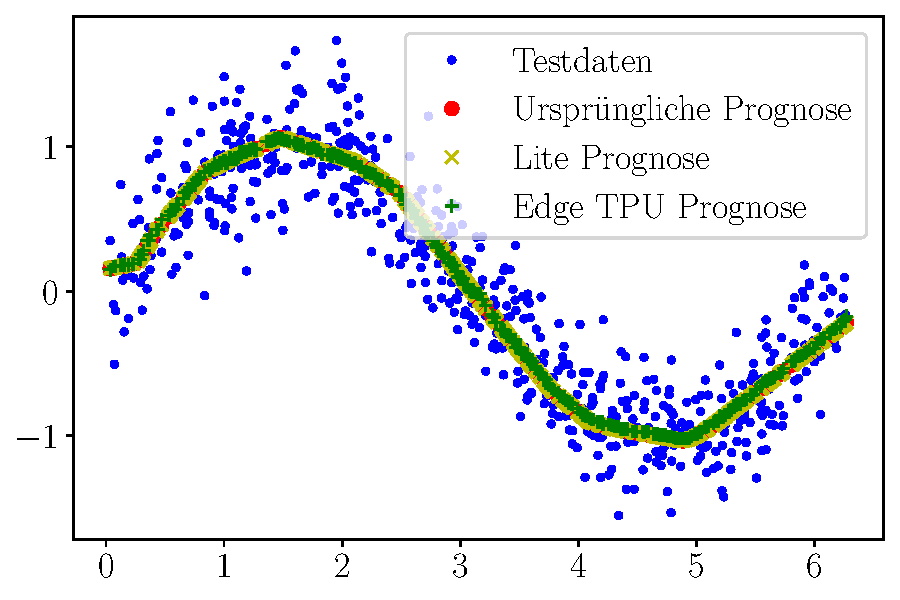
\includegraphics[width=\wMD]{first-nn/model-comparison.pdf}
  \caption{Ein Vergleich der Inferenzergebnisse des Keras-Modells, dem unquantisierten
  TFLite-CPU-Modell und dem quantisierten Edge-TPU-Modell}
  \label{fig:model-comparison}
\end{figure}
Es ist zu sehen, dass durch die Quantisierung keine oder nur kaum
zu bemerkende Genauigkeitsverluste entstanden sind.


\section{Ein Vergleich der Inferenzgeschwindigkeiten}
Die Inferenzgeschwindigkeiten der verschiedenen TFLite-Modelle
sollen nun verglichen werden. Hierfür kann das folgende Python-Programm
ausgeführt werden.
Das Gerät benötigt eine funktionierende Edge TPU
und das Python-Skript muss Zugriff auf
das \pythoninline{tflite_runtime} Paket haben.
Die Installation ist je nach Plattform eine unterschiedliche
(siehe hierfür die Coral AI und TensorFlow Dokumentation).
\begin{pythoncode}
import time
import tflite_runtime.interpreter as tflite
import platform
import numpy as np

EDGETUP_LIB = {
    "Linux": "libedgetpu.so.1",
    "Darwin": "libedgetpu.1.dylib",
    "Windows": "edgetpu.dll",
}[platform.system()]

# Die drei zu vergleichenden Modelle
sine_model_cpu = tflite.Interpreter("sine_model.tflite")
sine_model_quant_cpu = tflite.Interpreter("sine_model_quant.tflite")
sine_model_tpu = tflite.Interpreter(
    "sine_model_quant_edgetpu.tflite",
    experimental_delegates=[tflite.load_delegate(EDGETUP_LIB)],
)

sine_model_cpu.allocate_tensors()
sine_model_quant_cpu.allocate_tensors()
sine_model_tpu.allocate_tensors()

rng = np.random.default_rng(42)

def measure_performance(model):
    input_details = model.get_input_details()[0]
    input_index = input_details["index"]
    input_shape = input_details["shape"]
    dtype = input_details["dtype"]

    # 20000 Testdaten im Bereich null bis sechs
    test_data = rng.random(size=[20000, *input_shape], dtype=np.float32) * 6

    if dtype == np.int8:
        # Skaliere die Eingaben für quantisierte Modelle
        input_scale, input_zero_point = input_details["quantization"]
        test_data = test_data / input_scale + input_zero_point
        test_data = test_data.astype(dtype)

    result = 0
    for i, value in enumerate(test_data):
        model.set_tensor(input_index, value)
        # Messe die Zeit in Millisekunden
        start = time.perf_counter()
        model.invoke()
        inference_time = (time.perf_counter() - start) * 1000
        # Überspringe die ersten Messungen,
        # damit vom Cache Gebrauch gemacht werden kann
        if i > 10:
            result += inference_time
    return result

result = measure_performance(sine_model_cpu)
print(f"CPU Inferenzgeschwindigkeit: {result:.4f} ms")
result = measure_performance(sine_model_quant_cpu)
print(f"CPU quantisierte Inferenzgeschwindigkeit: {result:.4f} ms")
result = measure_performance(sine_model_tpu)
print(f"TPU Inferenzgeschwindigkeit: {result:.4f} ms")
\end{pythoncode}
Die folgenden Befehle zeigen wie der obere Benchmark durchgeführt werden kann.
In diesem Beispiel wurde der Test auf dem Siemens SIMATIC IOT2050 \eqref{fig:iot2050}
ausgeführt:
\begin{consolecode}
$ mkdir benchmark
$ cd benchmark
$ python3 -m venv --system-site-packages env
$ source env/bin/activate
$ pip install -U pip
$ pip install --ignore-installed numpy
$ wget "https://raw.githubusercontent.com/JensDll\
> /bachelorarbeit-notebooks/1.0.5/first-nn/benchmark/download.sh"
$ # Führe das Bash-Skript aus um die Modelle herunterzuladen
$ bash download.sh 1.0.5
$ cd models
$ python sine_benchmark.py
CPU Inferenzgeschwindigkeit: 492.3875 ms
CPU quantisierte Inferenzgeschwindigkeit: 452.9881 ms
TPU Inferenzgeschwindigkeit: 4490.2631 ms
\end{consolecode}
Die Zeiten zeigen ein überraschendes Ergebnis.
Das Modell, welches auf der Edge TPU ausgeführt wird, scheint um einiges
langsamer zu sein als die, welche auf der CPU ausgeführt werden.
Um zu bestätigen, dass die Edge TPU korrekt arbeitet,
können wir einen weiteren Benchmark durchführen,
aber dieses Mal mit einem Modell, welches bereits
getestete gute Inferenzgeschwindigkeiten besitzt. Wir
verwenden das in \autoref{fig:ui-classification-example}
gezeigte Modell, um Insektenbilder zu unterscheiden:
\begin{pythoncode}
import time
import tflite_runtime.interpreter as tflite
import platform
import numpy as np

EDGETUP_LIB = {
    "Linux": "libedgetpu.so.1",
    "Darwin": "libedgetpu.1.dylib",
    "Windows": "edgetpu.dll",
}[platform.system()]

# Die zu vergleichenden Modelle
insect_model_cpu = tflite.Interpreter("mobilenet_v2_1.0_224_inat_insect_quant.tflite")
insect_model_tpu = tflite.Interpreter(
    "mobilenet_v2_1.0_224_inat_insect_quant_edgetpu.tflite",
    experimental_delegates=[tflite.load_delegate(EDGETUP_LIB)],
)

insect_model_cpu.allocate_tensors()
insect_model_tpu.allocate_tensors()

rng = np.random.default_rng(42)

def measure_performance(model):
    input_details = model.get_input_details()[0]
    input_index = input_details["index"]
    input_shape = input_details["shape"][1:]

    # Zufälliges Testbild
    test_data = rng.integers(low=0, high=256, size=[1, *input_shape], dtype=np.uint8)

    result = 0
    for i in range(12):
        model.set_tensor(input_index, test_data)
        # Messe die Zeit in Millisekunden
        start = time.perf_counter()
        model.invoke()
        inference_time = (time.perf_counter() - start) * 1000
        # Überspringe die ersten zwei Messungen
        if i > 1:
            result += inference_time
    return result

result = measure_performance(insect_model_cpu)
print(f"CPU Inferenzgeschwindigkeit: {result:.4f} ms")
result = measure_performance(insect_model_tpu)
print(f"TPU Inferenzgeschwindigkeit: {result:.4f} ms")
\end{pythoncode}
Wurden die vorherigen Befehle ausgeführt, kann auch dieser Test einfach durchgeführt
werden:
\begin{consolecode}
$ python mobilenet_benchmark.py
CPU Inferenzgeschwindigkeit: 2025.3505 ms
TPU Inferenzgeschwindigkeit: 27.4516 ms
\end{consolecode}
Die Edge TPU zeigt ein deutlich besseres Ergebnis.
Der Gründe für die langsamere Geschwindigkeit im ersten Benchmark
sind unklar. Es gibt Diskussionen auf dem Google Coral
GitHub Repository (wie
\href{https://github.com/google-coral/edgetpu/issues/89}{\#89}), in denen
ähnliche Ergebnisse gezeigt werden.
Die Edge TPU scheint für Netze mit vielen vollständig verbundenen Schichten
langsamer zu sein als die Ausführung desselben Netzes auf der CPU.
Wird die TPU hingegen für andere Netzarchitekturen
eingesetzt (wie, dem \textit{Convolutional Neural Network} für \textit{Computer Vision}
im zweiten Test), führt dies zu einer wesentlich besseren Leistung.
Ein entwickeltes Modell sollte also immer zusammen
mit der verwendeten Hardware getestet werden, um die
Leistungsverbesserungen abzuschätzen und das mit der besten Geschwindigkeit auszuwählen.
Werden die oben durchgeführt Benchmarks vier weitere Male ausgeführt, ergeben sich
die Inferenzgeschwindigkeiten wie in \autoref{tab:benchmark-results}
zu sehen sind.
\begin{table}[h!]
  \centering
  \caption{Ein Vergleich der Inferenzgeschwindigkeiten, nachdem die
  gezeigten Benchmarks viermal hintereinander durchgeführt wurden}
  \label{tab:benchmark-results}
  \begin{tabular}{lSSSS}
    \toprule
                          & \multicolumn{4}{c}{Durchlauf (\unit{\milli\second})} \\ \cmidrule(){2-5}
    Modell                & 1         & 2         & 3         & 4                \\ \midrule
    Sinus CPU             & 490.9770  & 494.2958  & 500.0013  & 499.6144         \\
    Sinus quantisiert CPU & 448.8091  & 458.9007  & 456.8160  & 453.6806         \\
    Sinus Edge TPU        & 3958.7869 & 4466.2854 & 4329.7590 & 4392.6025        \\ \midrule
    MobileNet V2 CPU      & 2032.3503 & 2021.8814 & 2031.3118 & 2023.9531        \\
    MobileNet V2 Edge TPU & 27.5456   & 27.4322   & 27.5093   & 27.6126          \\ \bottomrule
  \end{tabular}
\end{table}
\chapter{Eine Anwendung für mobiles Maschinelles Lernen}
\label{chap:application}
Jetzt, wo ein Netz trainiert, bewertet,
in das TensorFlow Lite Format gewandelt und verglichen wurde,
heißt es das ausgewählte Modell in der Praxis einzusetzen.
Ein neuronales Netz allein, welches hervorragende Prognosen
macht, reicht jedoch nicht, um ein nützliches Produkt zu entwickeln:
Das Modell muss in einer Anwendung integriert werden, sodass
der Benutzer oder andere Teile des Systems
mit den Modellergebnissen interagieren können.
Der Entwurf einer solchen Anwendung ist die
Fokussierung dieses Kapitels.

\section{Die allgemeine Architektur auslegen}
Wie in \autoref{sec:problem-description} beschrieben wurde, ist es
typischerweise eine gute Idee, das Modell in einen Service zu verpacken.
Andere Teile der Anwendung können so jederzeit auf die Vorhersagen
des Netzes zugreifen. Dies ermöglicht es, neue Versionen
einzuspielen, ohne die Hauptanwendung zu unterbrechen.
Zusätzlich kann die Entwicklung flexibler gestaltet werden,
da es keine Einschränkung auf bestimmte Technologien
und Programmiersprachen gibt. Es kann so jederzeit das
beste Werkzeug für das zu lösende Problem ausgewählt werden.
Der Dienst, welcher das Modell ausführt, könnte in Python oder \cpp{}
geschrieben sein, und obwohl es möglich ist, Benutzeroberflächen 
in Python zu entwerfen, ist \cpp{} wahrscheinlich nicht das
richtige Hilfsmittel für diese Aufgabe.
Besser wäre es womöglich eine Sprache für das Web auszuwählen, 
wie zum Beispiel JavaScript.
\autoref{fig:app-architecture} zeigt die Architektur der Anwendung.
\begin{figure}[h!]
  \centering
  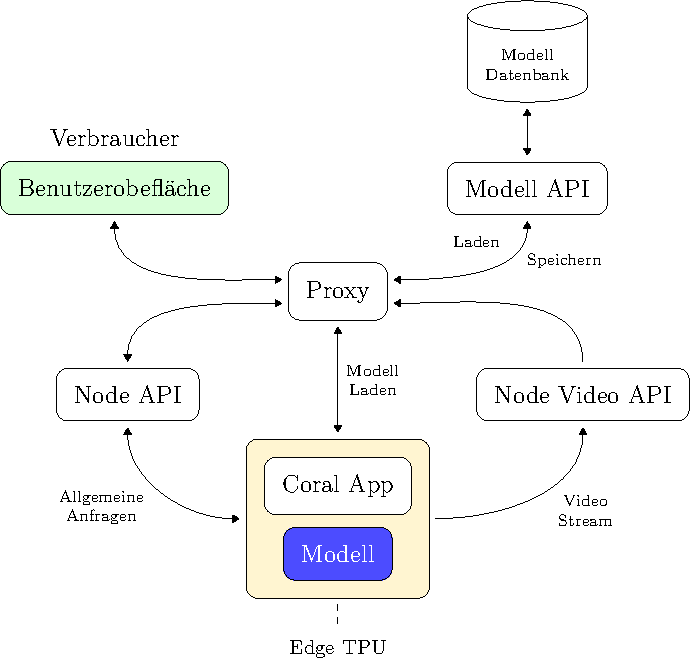
\includegraphics[width=\wLG]{app/app-architecture.pdf}
  \caption{Die Architektur der Anwendung: Ein Modell, das als Dienst
  bereitgestellt wird und verschiedene Services, die mit diesem kommunizieren}
  \label{fig:app-architecture}
\end{figure}

\noindent
Jedes Objekt mit einer Pfeilspitze spiegelt einen Service wieder, insgesamt sind
es sieben Stück. Ein Service ist eine unabhängige, wenn möglich kleine und
unkomplizierte Anwendung, welche nicht mehr als eine Aufgabe übernimmt.
Um die Verwaltung dieser Services zu erleichtern, wird Docker eingesetzt.
Jeder Dienst kann so isoliert in seinem eigenen Docker-Container ausgeführt
und über Docker-Netzwerke verbunden werden.\\[8pt]
Docker ist eine Freie Software, welche auf Linux, Windows und macOS
läuft. Sie erstellt und verwaltet Container
und kann diese sogar orchestrieren.
Docker, Inc., gegründet in 2008 (ursprünglich \textit{dotCloud} und später unter
dem Spitznamen \enquote{Docker}), ist das Unternehmen,
welche die Software entwickelt hat \parencite{onlide:docker-inc}.
Das Wort \enquote{Docker} kommt aus dem Englischen
und bedeutet \textit{\underline{dock} work\underline{er}} --
eine Person im Hafen die Schiffe be- und entlädt.
Es ermöglicht das einfache Teilen von Software
durch Docker-Images (einschließlich aller Abhängigkeiten
und in der Regel geeigneter Standardkonfiguration) und kann
diese mithilfe der Docker-Engine ausführen.
Wird ein Image ausgeführt, erstellt die Engine einen Docker-Container,
mit dem die Anwendung gut isoliert vom restlichen System gestartet wird.
Es ist ähnlich wie eine virtuelle Maschine,
nur viel schneller und schlanker, 
da der Container direkt auf dem Kernel des Hostbetriebssystems aufsetzt
\parencite[11-14]{book:docker-dd} \parencite[672]{book:hands-on-ml}.\\[8pt]
Docker eignet sich somit gut, um eine Anwendung mit der in dieser Arbeit beschriebenen
Zielsetzung zu entwickeln, die jeder herunterladen und mit ein paar Befehlen
auf dem eigenen System ausführen kann. Der Quelltext zur Anwendung
sowie die bisherigen Programmausschnitte
befinden such auf dem GitHub-Profil des Autors.
Die Docker-Images der in \autoref{fig:app-architecture} zu sehenden
Services sind über Docker Hub verfügbar.
Docker Hub ist eine Plattform zum Teilen von Docker-Images und das als Standard
eingestellte Image-Register einer neuen Installation der Docker Software.
Ein Image-Register enthält ein oder mehrere Image-Repositorys
und diese enthalten wiederum ein oder mehrere Images.
Die folgenden Punkte fassen die wichtigsten Links zusammen:
\begin{itemize}
  \item Der Quelltext zur Anwendung auf GibHub
        (\url{https://github.com/JensDll/coral-ml}).
  \item Die bisherigen Programme und Ausschnitte zum Erstellen der Abbildungen
        (\url{https://github.com/JensDll/bachelorarbeit-notebooks}).
  \item Die Docker-Images der Services auf Docker Hub
        (\href{https://hub.docker.com/repository/docker/jensdll/coral-ml}
        {https://hub.docker.com/reposito\allowbreak ry/docker/jensdll/coral-ml}).
\end{itemize}

\section{Herunterladen der Dienste}
Um ein Image von Docker Hub herunterzuladen, wird
der \consoleinline{docker pull} Befehl verwendet.
Für offizielle Image-Repositorys nimmt dieser Befehl die folgende Form an:
\begin{consolecode}
$ docker pull <repository>:<tag>
\end{consolecode}
Es wird das Repository zusammen mit dem gewünschten Image
in der Form eines Tags angegeben.
Offizielle Repositorys sind ein Prinzip von Docker Hub.
Hier befinden sich von Docker Inc. ausgewählte
Images, die speziell geprüft, getestet,
gut dokumentiert und sicher sein sollten.
Die meisten populären und etablierten Anwendungen
und Betriebssysteme haben ihre eigenen
offiziellen Repositorys.
Diese sind Teil der obersten Ebene des Docker Hub Namensraums.
Das Abrufen von Images aus inoffiziellen Repositorys
ist im Wesentlichen dasselbe, hierfür
muss dem Repository-Namen
lediglich den Docker Hub Benutzernamen oder die Organisation
vorangestellt werden.
Der folgende Befehl lädt zum Beispiel das neuste
Benutzeroberflächen-Image aus dem \consoleinline{coral-ml}
Repository herunter, das der Person gehört, deren Docker Hub Benutzername
\consoleinline{jensdll} ist:
\begin{consolecode}
$ docker pull jensdll/coral-ml:vue-app_latest
513c6babab2b: Pull complete
e0fc2ec040ad: Pull complete
b80eb69b3b2a: Pull complete
6b9432260a23: Pull complete
3e07e4cdac0e: Pull complete
e0984574aa06: Pull complete
7504b347e849: Pull complete
d8102b350cfa: Pull complete
a1e035743dcc: Pull complete
Digest: sha256:dc255cc3b2...14260180b2
Status: Downloaded newer image for jensdll/coral-ml:vue-app_latest
docker.io/jensdll/coral-ml:vue-app_latest
\end{consolecode}
Hier befinden sich alle Dienste der Anwendung.
Der Befehl \consoleinline{docker images} gibt Auskunft über die zur Zeit auf dem Host
verfügbaren Images, hier ist die neu geladene Anwendung nun zu sehen:
\begin{consolecode}
$ docker images
REPOSITORY         TAG              IMAGE ID       CREATED        SIZE
jensdll/coral-ml   vue-app_latest   3328de4e34a8   34 hours ago   126MB
\end{consolecode}
Derselbe Befehl kann auch für die restlichen Services ausgeführt werden:
\begin{consolecode}
$ docker pull jensdll/coral-ml:mariadb_latest
$ docker pull jensdll/coral-ml:record-api_latest
$ docker pull jensdll/coral-ml:node-api_latest
$ docker pull jensdll/coral-ml:node-video_latest
$ docker pull jensdll/coral-ml:proxy_latest
$ docker pull jensdll/coral-ml:coral-app_latest
\end{consolecode}
Das Docker-Image der Modell API trägt den Namen \consoleinline{record-api},
da dort neben den Modelldateien auch andere Informationen gespeichert werden,
wie zum Beispiel die Bezeichnungen der Klassen
für Klassifizierungsaufgaben in Form von Text- oder CSV-Dateien.
Ein Ausschnitt einer solchen Datei könnte wie folgt aussehen:
\begin{consolecode}
$ # Klassifizierung von Insektenbildern
$ cat labels.txt
Coccinella septempunctata (Seven-spotted Ladybird)
Zanclognatha jacchusalis (Wavy-lined Zanclognatha Moth)
[...]
Thasus neocalifornicus (Giant Mesquite Bug)
Palpita quadristigmalis (Four-spotted Palpita)
\end{consolecode}
Der Download der restlichen Dienste sollte nun abgeschlossen sein.
Ein erneuter Blick auf die verfügbaren Images führt zu folgendem Ergebnis:
\begin{consolecode}
$ docker images
REPOSITORY         TAG                 IMAGE ID       CREATED             SIZE
jensdll/coral-ml   vue-app_latest      ca8f49bae427   About an hour ago   126MB
jensdll/coral-ml   record-api_latest   bfb1e0f29b8b   About an hour ago   216MB
jensdll/coral-ml   coral-app_latest    8c9e9d79a019   About an hour ago   1.51GB
jensdll/coral-ml   node-api_latest     747e9d9c033c   About an hour ago   194MB
jensdll/coral-ml   node-video_latest   f184084a9639   About an hour ago   172MB
jensdll/coral-ml   mariadb_latest      0a215d70439a   About an hour ago   743MB
jensdll/coral-ml   proxy_latest        2ee77b530075   About an hour ago   126MB
\end{consolecode}

\section{Starten und Verbinden der Dienste}
Jetzt wo alle nötigen Images heruntergeladen sind, können
sie verwendet werden um die Anwendung zu starten.
\autoref{fig:container-image-relation} zeigt
die allgemeine Beziehung zwischen Docker-Image und Container.
\begin{figure}[h!]
  \centering
    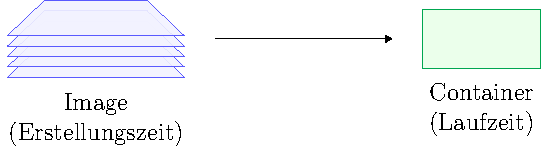
\includegraphics[width=\wMD]{app/container-image-relation.pdf}
    \caption{Die allgemeine Beziehung zwischen
    Docker-Image und Container \parencite[52]{book:docker-dd}}
    \label{fig:container-image-relation}
\end{figure}

\noindent
Die Befehle \consoleinline{docker run}, \consoleinline{docker service create}
und \consoleinline{docker create} zusammen mit
\consoleinline{docker start} werden verwendet,
um ein oder mehrere Container von einem Image zu starten.
Nachdem ein Container erstellt wurde,
ist dieser fest an das zugrunde liegende Image gebunden.
Das Image kann erst dann gelöscht werden,
wenn es keine Container mehr gibt, die dieses verwenden.
Der Versuch, ein Image mit noch verbundenen Containern zu entfernen, führe zu einem Fehler.
Die Docker-Images der Anwendung sind alle zusammen kompatibel mit der ARM64-Architektur
und können daher vollständig auf einem Gerät wie dem
Siemens SIMATIC IOT2050 ausgeführt werden.
Das Bereitstellen einer containerisierten Anwendung ist ein zweiteiliger Prozess:
\begin{enumerate}
  \item Erstelle ein Netzwerk über das die Container kommunizieren.
  \item Lege die Container an, starte und verbinde sie mit dem Netzwerk.
\end{enumerate}
Wird die Anwendung auf einem einzelnen Host ausgeführt, bietet sich
die einfachste Form der Docker-Netzwerke an: dem \textit{single-host bridge network}.
Der Name verrät bereits zwei Dinge \parencite[155]{book:docker-dd}:
\begin{description}[style=nextline]
  \item[Single-Host]
  Das Netz existiert auf einem einzigen Docker-Host und kann auch nur Container
  von diesem Host verbinden.
  \item[Bridge]
  Es handelt sich um eine Implementierung des 802.1d Bridge Standards (Layer-2-Switch).
\end{description}
Der folgende Befehl erstellt ein \textit{single-host bridge network} mit dem Namen
\consoleinline{appnet}:
\begin{consolecode}
$ docker network create --driver bridge appnet
\end{consolecode}
Dieses taucht nun in der Liste der Docker-Netze auf:
\begin{consolecode}
$ docker network ls
NETWORK ID     NAME      DRIVER    SCOPE
2a64863b85ac   appnet    bridge    local
de8bf5113652   bridge    bridge    local
[...]
\end{consolecode}
Zusätzlich wurde auf Linux eine neue \textit{Linux bridge} im Kernel angelegt.
Diese können mit dem \textit{bridge control} Befehl
aus dem \textit{bridge-utils} Paket beobachtet werden:
\begin{consolecode}
$ brctl show
bridge name       bridge id           STP enabled   interfaces
br-2a64863b85ac   8000.02421cd6ffff   no
docker0           8000.0242b48f93e6   no
\end{consolecode}
Die Ausgabe zeigt zwei Netzwerkbrücken. Die erste Zeile (\consoleinline{br-2a64863b85ac})
bezieht sich auf die neu angelegte Docker-Brücke \consoleinline{appnet}.
Die zweite Zeile (\consoleinline{docker0}) korrespondiert mit der
von Docker erstellten Standard-Brücke. Keine der beiden Brücken
haben verbundene Geräte (\consoleinline{interfaces} Spalte).
Es können nun Container erstellt werden:
Die folgenden Befehle starten zwei Container mit Basis auf dem
\textit{Alpine Linux} Docker-Image, welches nur rund \qty{5}{\mega\byte} groß ist,
verbinden sie mit der Brücke und führen das Kommando \consoleinline{sleep 1d} aus:
\begin{consolecode}
$ docker run -d --network appnet --name c1 alpine sleep 1d
$ docker run -d --network appnet --name c2 alpine sleep 1d
\end{consolecode}
Ein Blick in das \consoleinline{appnet} Netz offenbart zwei verbundene Container:
\begin{consolecode}
$ docker network inspect appnet
[...]
"Containers": {
  "341ee8dfafa...d0401892a7d": {
    "Name": "c1",
    "EndpointID": "ad3241d27a7...3ba94ca3225",
    "MacAddress": "02:42:ac:12:00:02",
    "IPv4Address": "172.18.0.2/16",
    "IPv6Address": ""
  },
  "8c574b9a71e...7fa033427e9": {
    "Name": "c2",
    "EndpointID": "0f2a5f0dcdd...8dd3d481861",
    "MacAddress": "02:42:ac:12:00:03",
    "IPv4Address": "172.18.0.3/16",
    "IPv6Address": ""
  }
}
[...]
\end{consolecode}
Auch das \consoleinline{brctl} Kommando zeigt nun zwei angeschlossene Interfaces:
\begin{consolecode}
$ brctl show
bridge name       bridge id           STP enabled   interfaces
br-2a64863b85ac   8000.02421cd6ffff   no            veth063da62
                                                    veth3c4e683
docker0           8000.0242b48f93e6   no
\end{consolecode}
Innerhalb einer der Container sollte es nun möglich sein, den jeweils
anderen Container per Name zu erreichen.
Dies funktioniert deshalb, da alle Container automatisch
beim eingebetteten Docker DNS Dienst registriert werden
und so die Namen aller Container
im selben Netzwerk auflösen können \parencite[160]{book:docker-dd}.
Die folgenden Befehle testen die Verbindung:
\begin{consolecode}
$ # Bringe eine Shell an Container c1 an
$ docker exec -it c1 sh
(c1) $ # Ein Ping zu Container c2 per Name gelingt
(c1) $ ping c2 -c 2
PING c2 (172.18.0.3): 56 data bytes
64 bytes from 172.18.0.3: seq=0 ttl=64 time=0.582 ms
64 bytes from 172.18.0.3: seq=1 ttl=64 time=0.279 ms
\end{consolecode}
Die Namensauflösung funktioniert, Docker konnte dem Containernamen automatisch
die richtige IP-Adresse zuordnen.
Dies wird die Grundlage sein, wenn es darum geht
die unterschiedlichen Teile der Anwendung zu verbinden.
Zuerst werden die noch laufenden Container angehalten und entfernt:
\begin{consolecode}
$ docker stop c1 c2
$ docker rm c1 c2
\end{consolecode}
Die Anwendungscontainer können nun erstellt werden
und die folgenden Punkte beschreiben die nötigen Befehle.
\paragraph{Benutzeroberfläche}\mbox{}
\begin{consolecode}
$ docker create --network appnet -p 8080:80 \
>   --name vue-app jensdll/coral-ml:vue-app_latest
\end{consolecode}
Bislang hieß es, dass Container auf
Netzwerkbrücken nur mit anderen Containern im selben Netz kommunizieren können.
Mit Port-Mapping kann diese Eigenschaft umgangen werden. Der Befehl
\consoleinline{-p 8080:80} weist der Docker Engine an, den
TCP-Port 8080 des Hosts an den TCP-Port 80 des Containers weiterzuleiten.
Die Benutzeroberfläche kann so von außerhalb über die IP-Adresse des Geräts
an Port 8080 abgerufen werden.
\paragraph{Datenbank}\mbox{}
\begin{consolecode}
$ docker create --network appnet \
>   -e MARIADB_ROOT_PASSWORD='Pwd12345!' \
>   --name mariadb jensdll/coral-ml:mariadb_latest
\end{consolecode}
Dieser Befehl erstellt die Datenbank. Über die Umgebungsvariable
\consoleinline{MARIADB_ROOT_PASSWORD} wird das Passwort des Root-Nutzers angeben,
welches für die spätere Verbindung der API verwendet wird.
\paragraph{Modell API}\mbox{}
\begin{consolecode}
$ docker create --network appnet \
>   -e ConnectionStrings:RecordDb=\
> 'Server=mariadb,3306;Database=RecordDb;User Id=root;Pwd=Pwd12345!;' \
>   --name record-api jensdll/coral-ml:record-api_latest
\end{consolecode}
Dieser Befehl erstellt den Container zur Datenbankkommunikation.
In der Verbindungszeichenfolge wird das zuvor verwendete Passwort eingetragen.
\paragraph{Proxy}\mbox{}
\begin{consolecode}
$ docker create --network appnet -p 80:80 \
>   --name proxy jensdll/coral-ml:proxy_latest
\end{consolecode}
Der Proxy-Server muss über das öffentliche Netz vom Verbraucher aus erreichbar sein,
weshalb ein Port-Mapping von Port 80 nach 80 angegeben wird.
\paragraph{Node API}\mbox{}
\begin{consolecode}
$ docker create --network appnet \
>   --name node-api jensdll/coral-ml:node-api_latest
$ docker create --network appnet  \
>   --name node-video jensdll/coral-ml:node-video_latest
\end{consolecode}
Diese beiden APIs sind sich sehr ähnlich und dienen nur
der internen Kommunikation. Es wird daher nur das Netzwerk und der Containername
angegeben.
\paragraph{Coral App}\mbox{}
\begin{consolecode}
$ docker create --network appnet \
>   --device /dev/video0 --device /dev/apex_0 \
>   --name coral-app jensdll/coral-ml:coral-app_latest
\end{consolecode}
Als letzter Befehl wird die Coral Anwendung erstellt.
Der Container benötigt Zugriff auf verschiedene Hardwarekomponenten,
dieser kann gesetzt werden durch die \consoleinline{--device} Option.
Die \consoleinline{/dev/video0} Anweisung ermöglicht das Lesen
einer Videoquelle (zum Beispiel einer angeschlossen Webcam)
und die \consoleinline{/dev/apex_0} Gerätedatei ist der
Google Coral Half-Mini PCIe Anschluss \eqref{fig:iot2050}.\\[12pt]
Als letzter Schritt müssen die Container nur noch gestartet werden,
die Startreihenfolge ist hierbei relevant:
\begin{consolecode}
$ docker start mariadb record-api node-api node-video vue-app proxy coral-app 
\end{consolecode}
Zum Beispiel muss der Proxy-Container nach den APIs aber noch vor der Coral-App
gestartet werden. Die Anwendung wird nun ausgeführt mit sieben Containern
verbunden über eine lokale Netzwerkbrücke. Ein Blick auf die laufenden
Container ergibt folgende gekürzte Ausgabe:
\begin{consolecode}
$ docker container ls
CONTAINER ID   COMMAND                   STATUS         PORTS                  NAMES
19098722b243   "python main.py"          Up 4 minutes                          coral-app
270ca2c11b2e   "dotnet RecordAPI.dll"    Up 4 minutes   80/tcp                 record-api
14b6ca1e7c7f   "node bundle.min.js"      Up 4 minutes   80/tcp, 8080/tcp       node-video
6fb6af012163   "node bundle.min.js"      Up 4 minutes   80/tcp                 node-api
c9c5901cbbb4   "/docker-entrypoint..."   Up 4 minutes   0.0.0.0:80->80/tcp     proxy
53926b215876   "docker-entrypoint..."    Up 4 minutes   3306/tcp               mariadb
1eb49121c3ff   "/docker-entrypoint..."   Up 4 minutes   0.0.0.0:8080->80/tcp   vue-app
\end{consolecode}
Die Datenbank benötigt eine kurze Zeit,
um ein Backup wiederherzustellen.
Es sollten solange keine Anfragen durchgeführt werden,
da der API-Container ansonsten abstürzen könnte.
10 bis 15 Sekunden Wartezeit sollten ausreichen, geht dennoch etwas schief,
kann der jeweilige Container mit
dem Befehl \consoleinline{docker restart} neu gestartet werden.
Die Benutzeroberfläche ist über die IP-Adresse des Geräts
auf Port 8080 erreichbar.
\autoref{fig:website-on-devices} zeigt verschiedene
Teile der Webseite und wie diese auf unterschiedlichen Endgeräten aussieht.
\newpage
\begin{figure}[h!]
  \centering
  \begin{tikzpicture}
    \node [] (ipad) {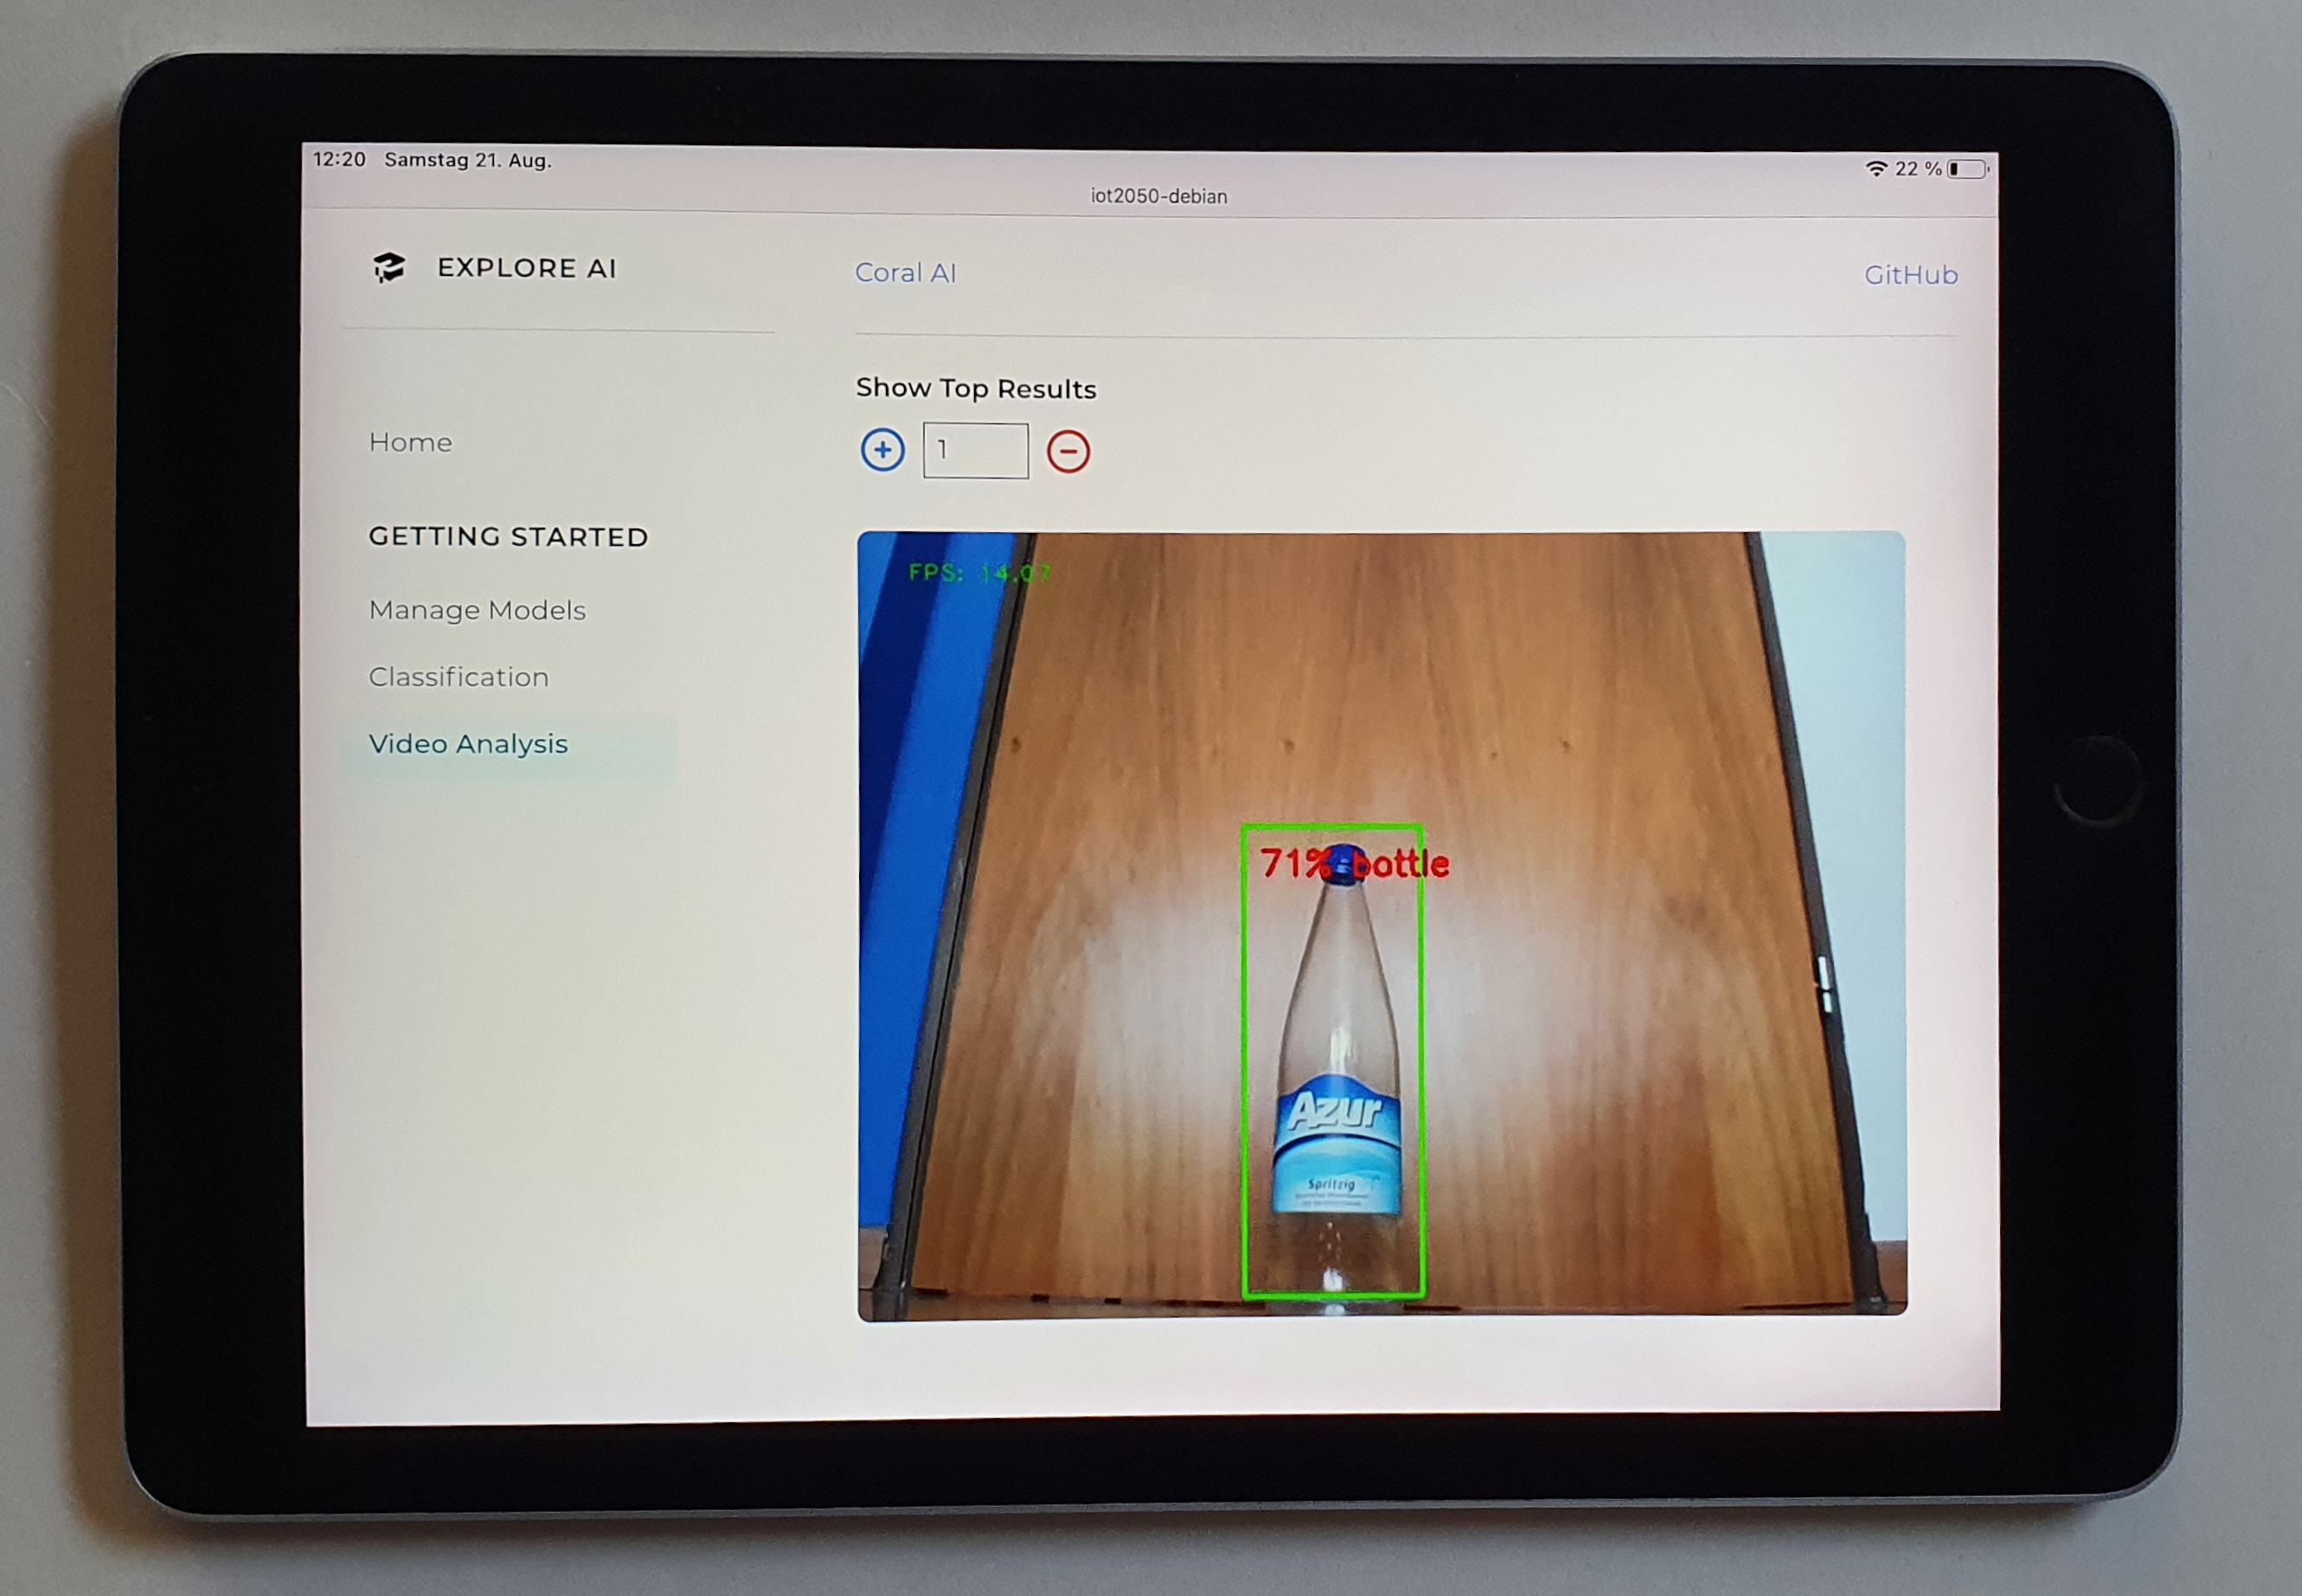
\includegraphics[width=\wMD]{app/ipad.png}};
    \node [below=5mm of ipad, xshift=-2.5cm]
      {\includegraphics[width=0.25\textwidth]{app/7s.png}};
    \node [below=5mm of ipad, xshift=2.5cm]
      {\includegraphics[width=0.22\textwidth]{app/5s.png}};
  \end{tikzpicture}
  \caption{Verschiedene Teile der Webseite und deren Aussehen auf unterschiedlichen Endgräten}
  \label{fig:website-on-devices}
\end{figure}

\noindent
Neben dem in \autoref{fig:ui-classification-example} gezeigten
Ausschnitt der Webseite zur Bildklassifizierung zeigen die
oberen Bilder den Videostream und die Verwaltung der verfügbaren
Modelle. Zum Zeitpunkt des Verfassens dieser Arbeit werden
verschiedenen Klassifizierungsmodelle und Objekterkennung
mit Video unterstützt. Bei den zu sehenden Netzen
handelt es sich um vom Coral-Team zur Verfügung gestellten
Demomodellen. Eine Erweiterung der Anwendung
durch zusätzliche Netzarchitekturen sollte
jedoch mit moderatem Aufwand möglich sein.
Das Video wird vom Aufnahmegerät über die Schnittstelle
an beliebig viele Verbraucher übertragen.
Auf dem IOT2050 wird hierbei eine
Bildwiederholrate von 10 bis \qty{15}{FPS} erreicht.
In Anbetracht der CPU Auslastung, welche durch die anderen
parallel laufenden Container entsteht,
reicht dies für flüssiges Video.
\chapter{Reflektion und Ausblick}
Die vorliegende Bachelorarbeit befasst sich mit der Frage
\enquote{Wie kann ein System entwickelt werden, mit dem verschiedene DL-Modelle
verwaltet werden können, welches modular und einfach erweiterbar ist
und Modellergebnisse über gemeinsame Schnittstellen im Netz kommuniziert?}
Um diese Frage zu beantworten, wurden
die Grundlagen von Deep Learning untersucht
und den Prozess beschrieben, wie mit TensorFlow und Keras
ein neuronales Netz erstellt und trainiert werden kann.
Anhand dieser Überlegung konnte schließlich die Architektur einer Anwendung
vorgestellt werden, mit der ein neuronales Netz in der Praxis eingesetzt wird.\\[8pt]
Das Modell wurde in ein mobil- und TPU-kompatibles Format umgewandelt
und anschließend miteinander vergleichen.
\autoref{fig:model-comparison} zeigt,
dass hierdurch keine oder nur kaum zu bemerkende Genauigkeitsverluste
entstanden sind.
Jedoch wird nach \autoref{fig:sine_model_inference_time}
das Ergebnis festgehalten,
dass zumindest bei kleinen Modellen und bestimmten Netzarchitekturen
die Inferenzgeschwindigkeit
auf der Edge TPU nicht unbedingt schneller ist als die gleiche Ausführung auf der CPU.
Es wird deshalb der Entschluss gefasst,
ein entwickeltes Netz immer zusammen mit der verwendeten Hardware zu testen,
um das mit den besten Ergebnissen auszuwählen.\\[8pt]
Die vorgestellte Anwendung \eqref{fig:app-architecture} besteht aus mehreren kleinen
Einheiten. Im Rahmen der Zielsetzung des System als ein Demoprojekt zu dienen
wurde eine Möglichkeit demonstriert,
wie diese mit Docker auf einem Gerät wie dem Siemens
SIMATIC IOT2050 bereitgestellt wird.\\[8pt]
Weitere Forschung und Entwicklung können auf diesen Ergebnissen
aufbauen. Es ist gut möglich die Anwendung zu erweitern oder
auch einzelne Dienste auszuwechseln.
Aktuell ist die Coral-Anwendung in Python geschrieben.
Um den Mehraufwand zu reduzieren, der dadurch entsteht ein
Python-Programm auszuführen, könnte diese in ein \cpp{}-Projekt
umgewandelt werden.
Dies sollte nicht nur die Leistung des Dienstes verbessern, sondern
auch die Imagegröße reduzieren.
\printbibliography[title = Literaturverzeichnis]
\addcontentsline{toc}{chapter}{Literaturverzeichnis}
\appendix
\chapter{Gradientenabstiegsverfahren}
\label{appx:gradient-descent}
Das Gradientenabstiegsverfahren oder einfach nur Gradientenverfahren
(engl. \textit{gradient decent})
ist ein allgemeiner Optimierungsalgorithmus
um eine Kostenfunktion zu minimieren \parencite[118]{book:hands-on-ml}.
Man stelle sich vor, man befinde sich auf einem Hügel im dichten Nebel
und möchte das Tal erreichen.
Eine gute Strategie wäre es, die Steigung des
Hügels abzuschätzen und sich dort entlangzubewegen,
wo die Senkung am größten ist.
Das Gradientenverfahren führt genau diese Schritte durch,
es misst die Steigung der Kostenfunktion für alle Parameter
und geht für jeden einen kleinen Schritt in die Richtung des Abhangs.
Betrachten wir eine einfache Kostenfunktion
mit nur einem Parameter:
\begin{equation*}
  J(x) = x^2 
\end{equation*}
Das Optimierungsproblem besteht darin, ein $x$ zu finden, mit dem die Funktion minimiert wird.
Die folgende Schritte beschreiben das Vorgehen:
\begin{enumerate}
  \item Wähle einen zufälligen Startpunkt $x$.
  \item Bestimme die Steigung der Funktion in diesem Punkt.
  \item Mache einen Schritt in Richtung des Abhangs und aktualisiere den $x$-Wert.
  \item Wiederhole Schritt zwei bis drei so lange,
        bis sich $x$ nicht mehr oder nur noch sehr wenig ändert.
\end{enumerate}
Um die Steigung zu bestimmen, muss die Ableitung der Kostenfunktion ermittelt werden.
\autoref{eq:one-step-gd-x2} zeigt einen Durchlauf der eben beschriebenen Schritte.
\begin{equation}
  x = x - \alpha \cdot \frac{\mathrm{d}J}{\mathrm{d}x} = x - \alpha \cdot 2x
  \label{eq:one-step-gd-x2}
\end{equation}
Der Parameter $\alpha$ beschreibt die Schrittweite. Diese wird auch das
Lerntempo genannt (engl. \textit{learning rate}).
Das Gradientenverfahren für unsere Beispielsfunktion kann in Python 
einfach umgesetzt werden:
\begin{pythoncode}
def dJ(x):
    return 2*x

def gradient_descent(start, n_epochs=50, learning_rate=0.01):
    x = start
    for _ in range(n_epochs):
        gradient = dJ(x)
        x = x - learning_rate * gradient
    return x
\end{pythoncode}
Die obere Funktion kann erweitert werden, um die Schritte anzuzeigen,
die der Algorithmus durchführt, wie in \autoref{fig:gd} zu sehen ist.
\begin{figure}[h!]
  \centering
  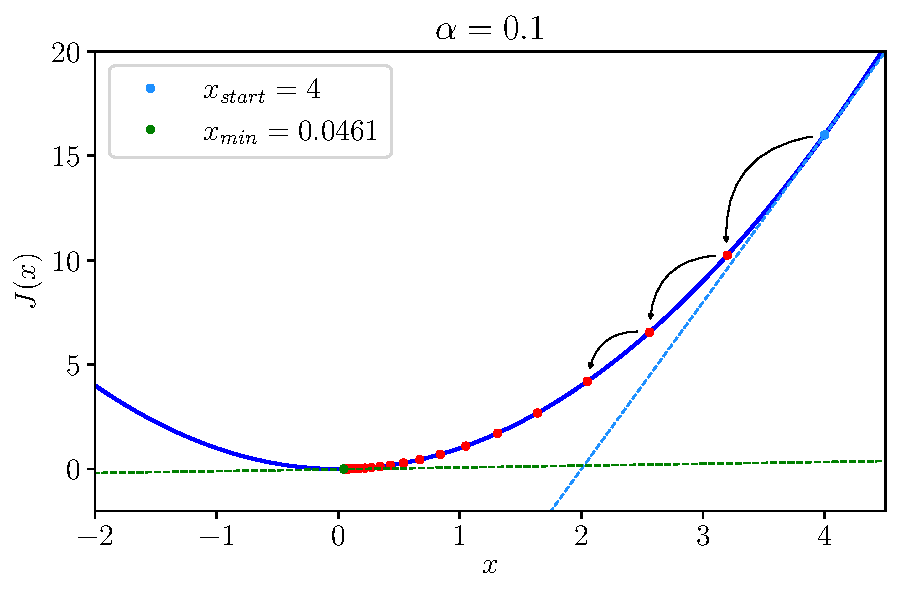
\includegraphics[width=0.75\textwidth]{gradient-decent/gd.pdf}
  \caption{Die ersten 20 Epochen des Gradientenabstiegs und einem Lerntempo von \num{0.1}}
  \label{fig:gd}
\end{figure}

\noindent
Die hellblau gestreifte Linie zeigt die Tangente der Funktion am Startpunkt und
die grün gestreifte Linie am Endpunkt. Nach 20 Epochen hat das Verfahren
den Tiefpunkt der Funktion (bei $x = 0$) fast erreicht.
Wird die Epochenzahl höher eingestellt, kann sich dem Tiefpunkt weiter angenähert werden:
\begin{pyconcode}
>>> x_min = gradient_descent(start=100, n_epochs=1000, learning_rate=0.1)
>>> x_min
1.2302319221611203e-95
\end{pyconcode}
Das Lerntempo ist ein wichtiger Parameter, der ausschlaggebend ist,
wie schnell ein gegebenes Modell trainiert werden kann.
Ist das Lerntempo zu klein, dauert das Training lange,
da der Gradientenabstieg insbesondere an Stellen mit geringer Steigung nur
winzige Schritte durchführt:
\begin{figure}[h!]
  \centering
  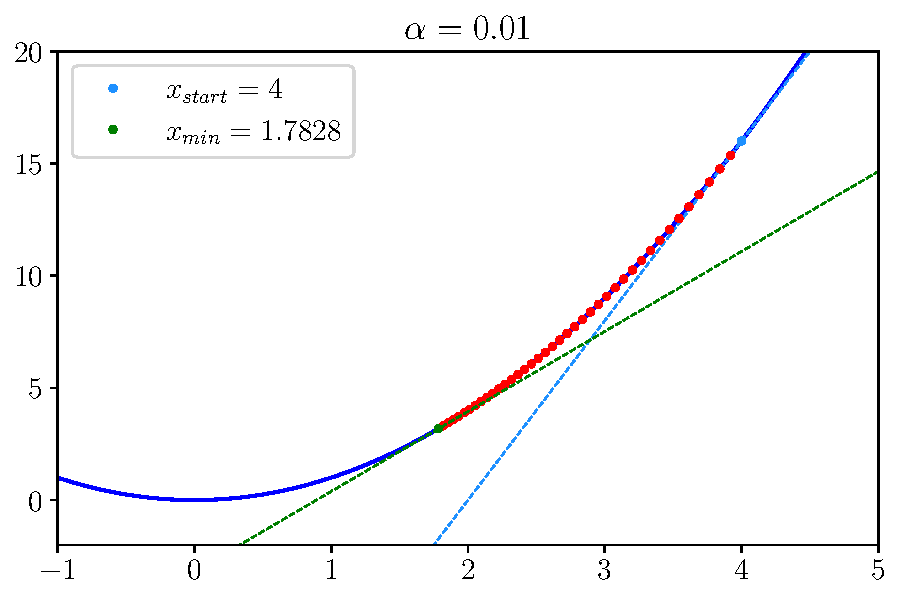
\includegraphics[width=0.75\textwidth]{gradient-decent/gd-low-lr.pdf}
  \caption{Die ersten 40 Epochen des Gradientenabstiegs und einem Lerntempo von \num{0.01}}
  \label{fig:gd-low-lr}
\end{figure}

\noindent
Ist das Lerntempo zu groß, kann es passieren, dass gar keine Lösung gefunden wird
und der $x$-Wert divergiert:
\newpage
\begin{figure}[h!]
  \centering
  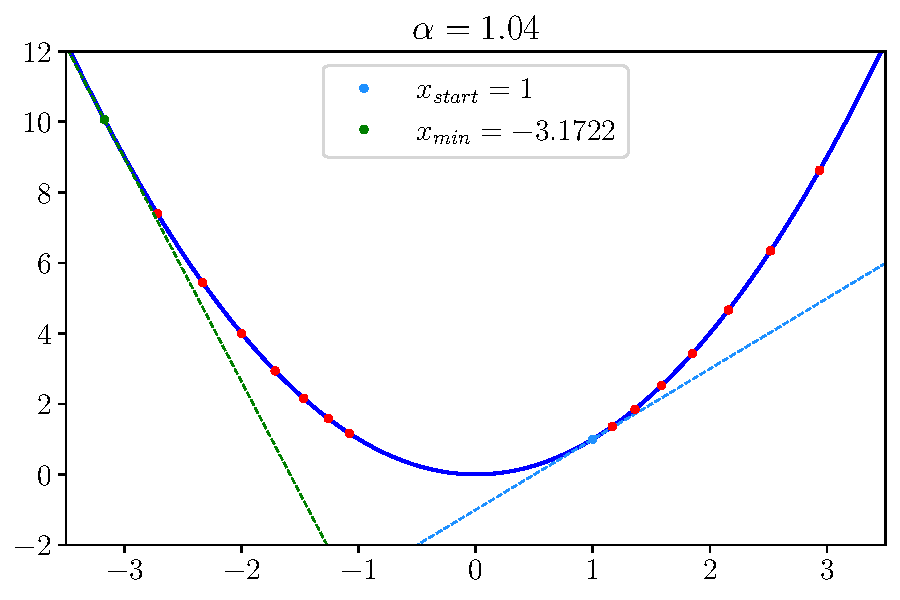
\includegraphics[width=0.75\textwidth]{gradient-decent/gd-high-lr.pdf}
  \caption{Die ersten 15 Epochen des Gradientenabstiegs und zu hohem Lerntempo}
  \label{fig:gd-high-lr}
\end{figure}

\noindent
Ein weiter Vorbehalt des Gradientenverfahrens liegt in der Kostenfunktion.
Nicht alle Kostenfunktionen haben eine so praktische Form wie im bisherigen Beispiel.
Betrachten wir den folgenden Fall:
\begin{figure}[h!]
  \centering
  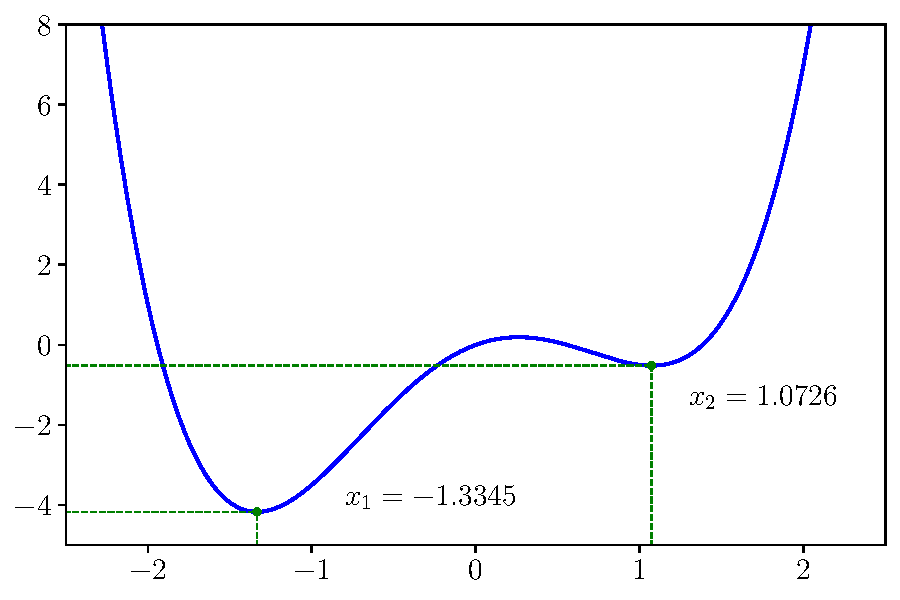
\includegraphics[width=0.75\textwidth]{gradient-decent/mulitple-minima.pdf}
  \caption{Kostenfunktion mit globalem und lokalem Minimum}
  \label{fig:mulitple-minima}
\end{figure}

\noindent
Die Funktion aus \autoref{fig:mulitple-minima} hat sowohl ein globales als auch auch
lokales Minimum. Ein Gradientenabstieg mit Startpunkt auf der rechten Seite würde
zwar einen Tiefpunkt finden, dieser ist jedoch nicht die bestmögliche Lösung des Problems.
\begin{figure}[h!]
  \centering
  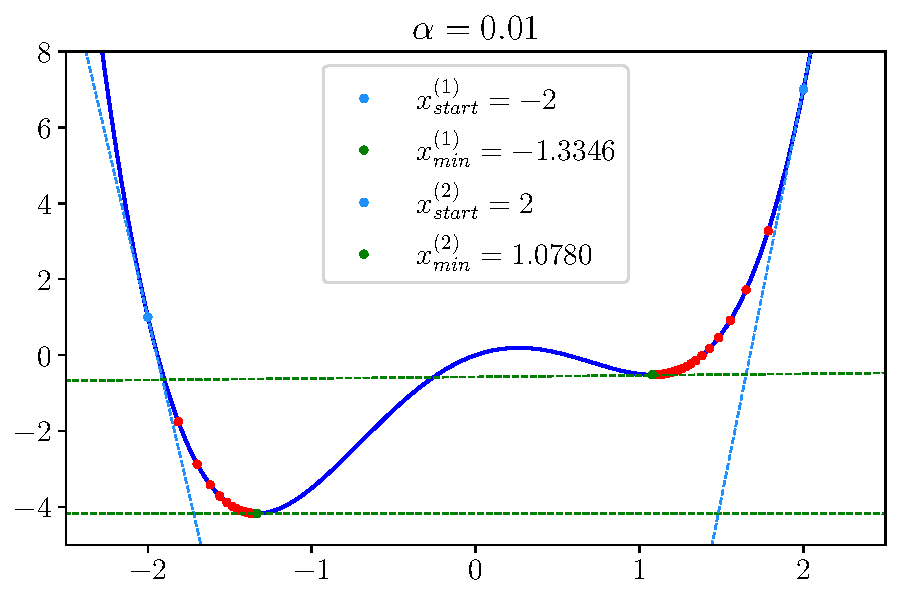
\includegraphics[width=0.75\textwidth]{gradient-decent/gd-mulitple-minima.pdf}
  \caption{Gradientenabstieg hängt im lokalen Minimum}
  \label{fig:gd-mulitple-minima}
\end{figure}

\noindent
Wie in \autoref{fig:gd-mulitple-minima} zu sehen ist, kann
der Gradientenabstieg in lokalen Minima hängen bleiben.
Für Kostenfunktionen mit mehr als einem Parameter
umfasst das Gradientenverfahren einige extra Schritte.
Für jeden zu trainierenden Parameter $\theta_{j}$ muss die
partielle Ableitung der Kostenfunktionen bestimmt werden
und diese wird verwendet, um den jeweiligen Parameter in einem Schritt anzupassen:
\begin{equation}
  \theta_{j} = \theta_j - \alpha \cdot \frac{\partial J}{\partial \theta_j}
\end{equation}


\end{document}